\documentclass[12pt,a4paper,oneside]{abntex2}
\usepackage[utf8]{inputenc}
\usepackage{amsmath}
\usepackage{esint}
\usepackage{amsfonts}
\usepackage{amssymb}
\usepackage{graphicx}
\usepackage{subfig}
\graphicspath{{fig/}}
\providecommand{\norm}[1]{\lVert#1\rVert}
\usepackage{empheq}

%\usepackage[alf ,abnt-etal-cite=2 , abnt-year-extra-label=yes , abnt-etal-list=0, abnt-etal-text=it]{abntex2cite}

%capa
\autor{DAVID DA COSTA DE PINHO}% introduz nome do autor
\titulo{FUNDAMENTOS DE MAGNETO-ELASTICIDADE}
\data{2018}
\local{MACA\'E}

%anverso da folha de rosto
\preambulo{Monografia apresentada ao Centro de Ci\^encia e Tecnologia da Universidade Estadual do Norte Fluminense, como parte das exig\^encias para aprova\c{c}\~ao no Exame de Qualifica\c{c}\~ao.}
\orientador{Viatcheslav Ivanovich Priimenko, Ph.D}
\tipotrabalho{monografia}

\begin{document}

\imprimircapa

\imprimirfolhaderosto%anverso

%{\ABNTEXchapterfont\Large\textsc{\imprimirautor}} - para aumentar a fonte e colocar em caixa alta

%importante dar enter para pular linha entre os tipos de textos

\begin{folhadeaprovacao}

\begin{center}
{\ABNTEXchapterfont\Large\bfseries\imprimirtitulo}\\\vspace{1cm}
{\ABNTEXchapterfont\Large\textsc{\imprimirautor}}

\end{center}

\vspace{1cm}
\hspace{.45\textwidth} \begin{minipage}{.5\textwidth}
\imprimirpreambulo
\end{minipage}

\vspace{1cm}
Trabalho aprovado em $\,7\,$ de Agosto de \imprimirdata.\\

\vspace{1cm}
Comiss\~ao Examinadora:\\
\assinatura{Prof. Marcia Miranda Azeredo, Ds.c - UENF}
\assinatura{Prof. André Duarte Bueno, Ds.c - UENF}
\assinatura{Prof. Fernando Diogo de Siqueira, Ds.c - UENF}
\assinatura{Prof. \imprimirorientador - UENF}

\begin{center}
\vfill
{\large\imprimirlocal}
\par
{\large\imprimirdata}
\end{center}

\end{folhadeaprovacao}

\begin{center}
{\ABNTEXchapterfont\Large\imprimirtitulo}\\\vspace{1cm}

\end{center}

\begin{resumo}
O objetivo principal desta obra \'e apresentar os fundamentos das teorias f\'isicas e matem\'atica relacionados ao efeito magneto-el\'astico, bem como um recondicionamento do modelo usado para descrever tal efeito. Inicialmente, apresentamos uma revis\~ao dos principais fen\^omenos pesquisados atualmente, envolvendo propaga\c{c}\~ao de ondas el\'asticas e eletromagn\'eticas. A mec\^anica do cont\'inuo e o eletromagnetismo s\~ao as duas teorias f\'isicas que descrevem a magneto-elasticidade, e introduzimos os principais conceitos dessas \'areas necess\'arios aos propositos desta monografia. Estudamos como ocorre o acoplamento entre ondas el\'asticas e eletromagn\'eticas bem como sua propaga\c{c}\~ao na subsuperf\'icie terrestre, atrav\'es de camadas estratigr\'aficas. Finalizamos com uma reescrita do modelo desse acoplamento de forma que possamos desenvolv\^e-lo analiticamente e produzir uma solu\c{c}\~ao num\'erica em trabalhos posteriores.

\vspace{\onelineskip} 
\noindent 
\textbf{Palavras-chave}: Magneto-Elasticidade, Mec\^anica do Cont\'inuo, Equa\c{c}\~oes de Maxwell.
\end{resumo}

\begin{center}
{\ABNTEXchapterfont\Large FOUNDATIONS OF MAGNETO-ELASTICITY}\\\vspace{1cm}
\end{center}

\begin{resumo}[Abstract]
\begin{otherlanguage*}{english}
The main purpose of this paper is present the foundations of physical and mathematical theories about magneto-elastic effect, and a reconditioning model to describe such effect. Firstly, we present a review of some phenomena found in current surveys, involving the propagations of elastic and eletromagnetics waves. Continuous mechanics and eletromagnetism describe magneto-elasticity, and we introduce a lots of required concepts from these areas to achieve the monography's goals. We also study how occurs the coupled propagation of elastic and eletromagnetics waves in Earth's subsurface, through stratigraphics layers. We finished rewriting the coupling's model in such manner that allow us to develope it analiticaly and to build a numerical solver in further works.

\vspace{\onelineskip} 
\noindent 
\textbf{Keywords}: Magneto-Elasticity, Continuous Mechanics, Maxwell's Equations.

\end{otherlanguage*}
\end{resumo}

\listoffigures

\newpage

\tableofcontents

\textual

\chapter{Introdução}
Esta monografia tem como finalidade principal o detalhamento da teoria que envolve o acoplamento de ondas eletromagnéticas e ondas elásticas que se propagam em meios estratificados, e homogêneos por camada, no subsolo terrestre. O desenvolvimento dessa teoria segue o modelo apresentado por \cite{erigen_1963} que trata da propagação de ondas elásticas num campo eletromagnético (geomagnético), onde essa propagação gera pequenas alterações geomagnéticas que se propagam, não com a velocidade da luz, mas ``acompanhando'' a onda elástica mantendo a velocidade desta última. 

A teoria é essencialmente uma combinação de elasticidade infinitesimal e teoria eletromagnética linearizada, e para torna o texto o mais auto-didata possível, serão apresentados nos capítulos \ref{sec.fund_eletr} e \ref{sec.fund_elast} os principais conceitos e definições acerca das teorias básicas sobre eletromagnetismo e elasticidade. 

Esta monografia faz parte de um conjunto de pesquisas que objetivam desenvolver um novo modelo matemático-computacional para descrever os fenômenos que envolvem a propagação simultânea de ondas eletromagnéticas e elásticas em subsuperfície, de modo que tal levantamento possa ser usado para aprimorar as técnicas de exploração de petróleo ou outro bem mineiral.
\chapter{Revis\~ao Bibliogr\'afica}

Em modelagem matem\'atica e computacional podemos realizar simula\c{c}\~oes num\'ericas e obter resultados te\'oricos os quais, muitas vezes, podem ser confrontados com os experimentos reais para auxiliar o estabelecimento da teoria que est\'a sendo desenvolvida. Desta forma, podemos verificar em \cite{surkov_97} a observa\c{c}\~ao de uma s\'erie de respostas eletromagn\'eticas e el\'asticas em meios geof\'isicos devidas a explos\~oes e terremotos:
\begin{enumerate}
\item anomalias locais no campo magn\'etico da Terra ap\'os explos\~ao;
\item efeitos de indu\c{c}\~ao devidos a ondas s\'ismicas (emitida por explos\~ao ou terremoto), onde os dist\'urbios geomagn\'eticos podem se propagar com a onda s\'ismica por longas dist\^ancias;
\item sondagem das caracter\'isticas mecano-el\'etricas da crosta utilizando ondas s\'ismicas (explos\~oes ou terremotos distantes);
\item estudo de dist\'urbios magn\'eticos de frequ\^encia muito baixa (ULF - Ultra Low Frequency) em regi\~oes sismicamente ativas.
\end{enumerate}
Podemos verificar tamb\'em a dedu\c{c}\~ao de f\'ormulas emp\'iricas que simulam numericamente as respostas observadas nesses experimentos. Os itens (1) e (2) s\~ao de maior import\^ancia para esta monografia e est\~ao detalhados a seguir.

\section{Efeito Sismo-Magn\'etico}

De acordo com \cite{stacey_64}, o campo magn\'etico residual observado pr\'oximo a uma explos\~ao no solo pode ser atribu\'ido ao efeito s\'ismico-magn\'etico, o qual consiste na magnetiza\c{c}\~ao ou desmagnetiza\c{c}\~ao de rochas compostas por elementos ferromagn\'eticos. O meio \'e magnetizado quando oscila durante a passagem de uma onda s\'ismica gerada por uma explos\~ao.

Para zona el\'astica, fora da zona de destrui\c{c}\~ao do meio perto da explos\~ao, existe uma rela\c{c}\~ao emp\'irica entre o incremento da magnetiza\c{c}\~ao $\Delta\,\mathbf{J}$ e a amplitude radial da tens\~ao $\tau_r$,
\begin{equation}\label{eq.momen_mag}
\Delta\,\mathbf{J}=\frac{\mathbf{J}\,\tau_r}{A},
\end{equation}
onde $\mathbf{J}$ \'e a magnetiza\c{c}\~ao inicial do meio e $A$ \'e um par\^ametro emp\'irico. O valor da tens\~ao $\tau_r$ diminui com a dist\^ancia $r$ a partir do ponto de explos\~ao de acordo com a rela\c{c}\~ao
\begin{equation}
\tau_r=\tau_*\frac{a_0}{r},
\end{equation}
onde $a_0$ \'e o raio da zona n\~ao el\'astica e $\tau_*$ \'e o limite de ruptura da rocha. Segundo \cite{surkov_89a}, podemos encontrar a solu\c{c}\~ao para a EDO \ref{eq.momen_mag} considerando que a tens\~ao depende do raio e obter as seguintes equa\c{c}\~oes para o campo magn\'etico residual,
\begin{align}\label{eq.camp_mag_empirico}
\mathbf{B}&=\frac{\mu_0\tau_*a_0}{2\,A\,r}\left(1-\frac{a_0^2}{r^2}\right)\left(\frac{3\,(\mathbf{J}\cdot \mathbf{r})\,\mathbf{r}}{r^2}-\mathbf{J}\right),\quad\text{se}\quad a_0\leq r\leq a,\\\nonumber\\
\mathbf{B}&=\frac{\mu_0\tau_*a_0(a^2-a_0^2)}{2\,A\,r^3}-\left(\frac{3\,(\mathbf{J}\cdot \mathbf{r})\,\mathbf{r}}{r^2}-\mathbf{J}\right),\quad\text{se}\quad r>a.
\end{align}
Onde $\mu_0$ \'e a permeabilidade magn\'etica no v\'acuo e $a$ \'e o raio da frente da onda el\'astica. Na figura \ref{fig.decai_camp_mag} podemos ver um gr\'afico cont\'inuo mostrando o decaimento do campo magn\'etico $\mathbf{B}(r)$ obtido num experimento de explos\~ao denominado \textit{MASSA}, utilizando TNT. Os detalhes desse experimento podem ser encontrados em \cite{yerzhanov_85}. Ainda na figura \ref{fig.decai_camp_mag}, podemos observar um gr\'afico tracejado mostrando o decaimento do campo magn\'etico atrav\'es de simula\c{c}\~oes num\'ericas, utilizando a equa\c{c}\~ao \ref{eq.camp_mag_empirico} com os seguintes par\^ametros: $\tau_*=0.1\,GPa$, $A=1\,GPa$, $a_0=100\,m$ e $J=0.12\frac{A}{m}$. A diferen\c{c}a entre as curvas em $r<0.5\,Km$ pode ser causada por outros mecanismos tamb\'em discutidos em \cite{surkov_97}.
\begin{figure}
\centering
\includegraphics[scale=.7]{grafico_campo_magnetico}
\caption{\textit{Decaimento do campo magn\'etico residual em fun\c{c}ao do raio. O gr\'afico cont\'inuo representa a decaimento medido ap\'os a explos\~ao MASSA e o gr\'afico tracejado \'e o resultado obtido atrav\'es de simula\c{c}\~oes num\'ericas.}}
\label{fig.decai_camp_mag}
\end{figure}

\section{Efeitos de Indu\c{c}\~ao devidos a Ondas S\'ismicas}

Altera\c{c}\~oes no campo geomagn\'etico podem ser geradas  pela passagem de uma onda s\'ismica emitida por terremoto ou explos\~ao, conforme preconizado por v\'arios autores como \cite{knopoff_55}, \cite{eringen_1963}, \cite{guglielmi_86a} e \cite{guglielmi_86b}. Essas altera\c{c}\~oes no campo geomagn\'etico podem viajar junto com a onda s\'ismica atrav\'es longas dist\^ancias, e s\~ao geradas por correntes de indu\c{c}\~ao j\'a que a onda el\'astica faz o meio condutivo oscilar na presen\c{c}a do campo geomagn\'etico. As equa\c{c}\~oes quasi-estacion\'arias de Maxwell descrevem esse efeito de indu\c{c}\~ao, onde a perturba\c{c}\~ao externa do campo geomagn\'etico acontece na vizinhanca da frente de onda s\'ismica e \'e dada por $\nabla\times(\mathbf{v}\times\mathbf{H}_0)$, onde $\mathbf{v}$ \'e a velocidade de deslocamento do meio e $\mathbf{H}_0$ \'e o campo geomagn\'etico. 

Segundo \cite{surkov_89b}, existem duas diferentes fases de espalhamento de correntes de indu\c{c}\~ao geradas por ondas s\'ismicas longitudinais se propagando em meios condutivos. A primeira fase se refere \`a perturba\c{c}\~ao geomagn\'etica que se espalha de acordo com leis da difusividade, ou seja, s\~ao mais r\'apidas que a frente de onda s\'ismica. A segunda fase come\c{c}a depois de determinado tempo, quando a onda s\'ismica longitudinal passa a se propagar junto com efeito de difus\~ao. Assim, a perturba\c{c}\~ao geomagn\'etica passa a se localizar na vizinhanca da frente de onda s\'ismica, com a velocidade desta. A perturba\c{c}\~ao geomagn\'etica se propaga um pouco \`a frente da onda s\'ismica, e \'e tratada como um esp\'ecie de precurssora. Na figura \ref{fig.onda_magnetoelastica} podemos observar uma perturba\c{c}\~ao na componente vertical do campo geomagn\'etico medida a uma dist\^ancia de $5\,Km$ da fonte, que neste exemplo \'e uma onda longitudinal emitida por explos\~ao no subsolo. A flecha indica a chegada da onda s\'ismica. \`A esquerda da flecha podemos observar a chegada de um precurssor magn\'etico, gerado pela difus\~ao da corrente de indu\c{c}\~ao excitada \`a frente da onda el\'astica. A amplitude desse precurssor decresce \`a medida que se afasta da frente de onda s\'ismica, a qual funciona como uma fonte din\^amica de perturba\c{c}\~ao geomagn\'etica.
\begin{figure}
\centering
\includegraphics[scale=1]{onda_magnetoelastica}
\caption{\textit{Perturba\c{c}\~ao da componente vertical do campo geomagn\'etico causada por uma onda s\'ismica longitudinal.}}
\label{fig.onda_magnetoelastica}
\end{figure}
Contudo, a detec\c{c}\~ao experimental de efeitos sismo-magn\'eticos n\~ao \'e uma tarefa f\'acil, de acordo com \cite{surkov_97}, porque o sinal de indu\c{c}\~ao seria camuflado pelo efeito sismogr\'afico, ou seja, a vibra\c{c}\~ao dos sensores magn\'eticos sob a\c{c}\~ao das ondas s\'ismicas. Assim, durante o tratamento das respostas, o sinal sismo-magn\'etico deve ser isoldado de ru\'idos e perturba\c{c}\~oes externas.

\section{Efeito Sismo-Magn\'etico e Terremotos}

As investiga\c{c}\~oes sismo-magn\'eticas desempenham um papel importante nas manifesta\c{c}\~oes de terremotos. Segundo \cite{Cukavac_2008}, levantamentos sismo-magn\'eticos repetitivos podem revelar varia\c{c}\~oes temporais nas propriedades das rochas devidas ao ac\'umulo de tens\~ao, e possivelmente, podemos observar altera\c{c}\~oes no campo geomagn\'etico em locais suscet\'iveis a terremotos. A distribui\c{c}\~ao dessas varia\c{c}\~oes, atrav\'es de medi\c{c}\~oes sucessivas, exibem padr\~oes de caracter\'isticas que podem estar relacionadas com a sismicidade do local durante um periodo de tempo. No entanto, se o levantamento dessas altera\c{c}\~oes pode ser considerado como o precurssor de um tereemoto, \'e ainda um tema controverso.

Uma possibilidade de investiga\c{c}\~ao \'e a compara\c{c}\~ao de dados sismo-magn\'eticos com dados geod\'esicos com o objetivo de investigar de forma eficaz a sismicidade de uma regi\~ao:
\begin{center}
For\c{c}as tect\^onicas. $\Rightarrow$\\
Deforma\c{c}\~ao de rochas. $\Rightarrow$\\
Aumento da deforma\c{c}\~ao. $\Rightarrow$\\
Altera\c{c}\~ao da magnetiza\c{c}\~ao das rochas (efeito piezo-magn\'etico). $\Rightarrow$\\
Altera\c{c}\~oes locais no campo geomagn\'etico.
\end{center}
Decadas de observa\c{c}\~oes de determinadas regi\~oes associadas \`as considera\c{c}\~oes teoricas tem rendido uma boa metodologia nos estudos tect\^onicos-magn\'eticos. \'E comumente aceito que uma rede de esta\c{c}\~oes de medi\c{c}~oes \'e necess\'aria para grava\c{c}\~ao dos fen\^omenos precursores de terremotos.

Uma dessas regi\~oes de investiga\c{c}\~ao \'e a Montanha Kopaonik, na S\'ervia, que \'e sismicamente ativa e foi alvo de levantamentos sismo-magn\'eticos por mais de vinte anos com magnetr\^onomos de $\pm\,0.2 nT$ de acur\'acia. Dentre os resultados encontrados podemos observar medi\c{c}\~oes realizadas no per\'iodo entre abril de 1983 e abril de 1984, com a ocorr\^encia de dois terremotos em setembro de 1983 com magnitudes 4.9 e 5.3. Na figura \ref{fig.camp_mag_ant_apo}, podemos observar algumas altera\c{c}\~oes no campo geomagn\'etico imediatamente antes e ap\'os esses dois terremotos. De acordo com \cite{Rikitake_80}, geralmente o padr\~ao das medi\c{c}\~oes seguem a regra de que a distribui\c{c}\~ao espacial do campo geomagn\'etico se altera em intervalos sucessivos de tempo, e as anomalias tendem a exibir sinais reversos enquanto o mapeamento espacial permanece mais ou menos o mesmo. Este fen\^omeno est\'a de acordo com os processos de acumula\c{c}\~ao de tens\~ao e relaxamento que ocorrem antes e ap\'os um terremoto e suporta a possibilidade de que a varia\c{c}\~ao observada no campo geomagn\'etico \'e de origem tect\^onica-magn\'etica.
\begin{figure}
\centering
\includegraphics[scale=.68]{camp_mag_antes_apos}
\caption{\textit{Altera\c{c}\~ao da intensidade do campo geomagn\'etico local antes e ap\'os dois terremotos.}}
\label{fig.camp_mag_ant_apo}
\end{figure}












\chapter{Fundamentos de eletromagnetismo}\label{sec.fund_eletr}

\section{Introdução}

\section{Fatos experimentais}

\subsection{Lei de Gauss para os fluxos elétrico e magnético}
De acordo com \cite{jackson_classical_1999} e \cite{sommerfeld_52} , os conceitos, definições e resultados em eletromagnetismo clássico partem das experiências de Cavendish e Coulomb no final do Séc. $XVIII$. A partir desses experimentos foi estabelecida a Lei de Coulomb
\begin{equation}\label{eq.forc_elet}
\textbf{F}=k\,\frac{q_1\,q_2}{||\textbf{x}_1-\textbf{x}_2||^2}\frac{\textbf{x}_1-\textbf{x}_2}{||\textbf{x}_1-\textbf{x}_2||},
\end{equation}
onde $q_i$ são as cargas elétricas (campos escalares) presentes nos pontos $\textbf{x}_i$, respectivamente, $k$ (campo escalar) é uma constante de proporcionalidade cujo valor depende do sistema de unidades de medida adotado, $||\textbf{x}_1-\textbf{x}_2||^2$ é a distância euclidiana entre as cargas e $\textbf{F}$ é a força elétrica exercida pela carga $q_1$ sobre a carga $q_2$. As notações em negrito representam campos vetorias pertencentes ao espaço $\mathbb{R}^3$, e o vetor normal que fornece a direção de interação entre as cargas é dado por $(\textbf{x}_1-\textbf{x}_2)/||\textbf{x}_1-\textbf{x}_2||$.

O campo elétrico $\textbf{E}$ é definido como sendo a força elétrica por unidade de carga em um determinado ponto que contém a carga de prova $q_2$, portanto é uma função vetorial que depende da posição da carga de prova em relação à carga fonte $q_1$, ou seja,
\begin{equation}\label{eq.camp_elet}
\textbf{E}=\lim_{q_2\to 0}\frac{\textbf{F}}{q_2}.
\end{equation}
A carga de prova foi tomada infinitesimalmente pequena para que o campo gerado por ela não perturbe a carga fonte. Experimentalmente, tanto a direção da força como a razão entre a força e a quantidade de carga vão se tornando constantes à medida que a quantidade de carga se torna cada vez menor, definindo a magnitude e a direção do campo elétrico. No SI, a unidade de medida de carga é o \textit{coulomb} $(C)$, o campo elétrico é o \textit{newton/coulomb} $(N/C)$ ou o \textit{volt/metro} $(V/m)$, e a constante $k=(4\pi\,\epsilon_0)^{-1}$ onde $\epsilon_0\simeq8.854\times10^{-12}$ é a \textit{permissividade elétrica no vácuo} medida em \textit{farad/m} $(F/m)$.

Substituindo a equação \ref{eq.camp_elet} em \ref{eq.forc_elet} temos que o campo elétrico agindo num ponto $\textbf{x}$ qualquer devido a uma carga $q_1$ no ponto $\textbf{x}_1$ é
\begin{equation}\label{eq.campo_eletrico}
\textbf{E}=k\,\frac{q_1}{||\textbf{x}_1-\textbf{x}||^2}\frac{\textbf{x}_1-\textbf{x}}{||\textbf{x}_1-\textbf{x}||},
\end{equation}
como podemos observar na figura \ref{fig.camp_eletr} simulando um sistema de coordenadas qualquer.
\begin{figure}[!htb]
\centering
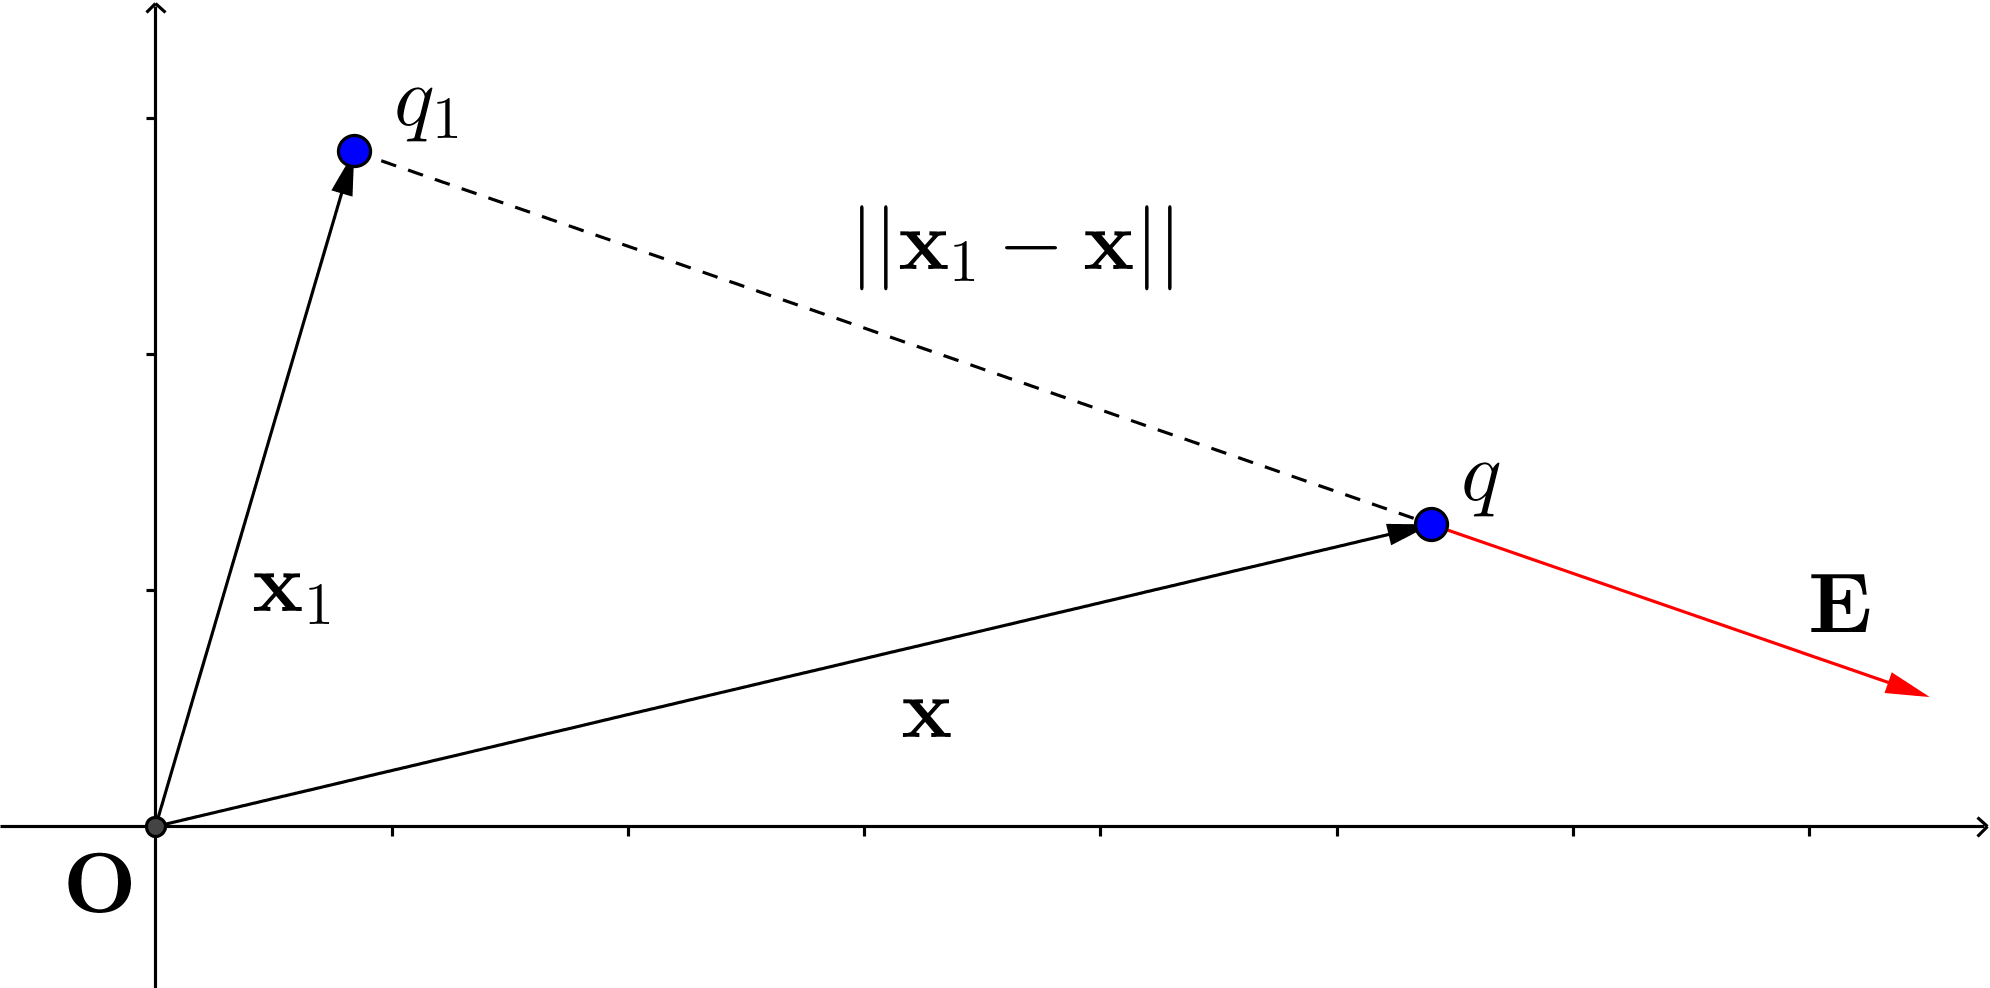
\includegraphics[scale=1.5]{camp_elet}
\caption{\textit{Exemplificação da interação entre cargas elétricas devido à geração, em função de $q_1$, de um campo elétrico. A força elétrica $\textbf{F}$ atuando numa carga qualquer $q$ tem mesma direção do campo elétrico $\textbf{E}$, com mesmo sentido ou sentido oposto conforme a carga $q$ é positiva ou negativa, respectivamente.}}
\label{fig.camp_eletr}
\end{figure}

%\begin{figure}[!htb]
%\centering
%\subfloat{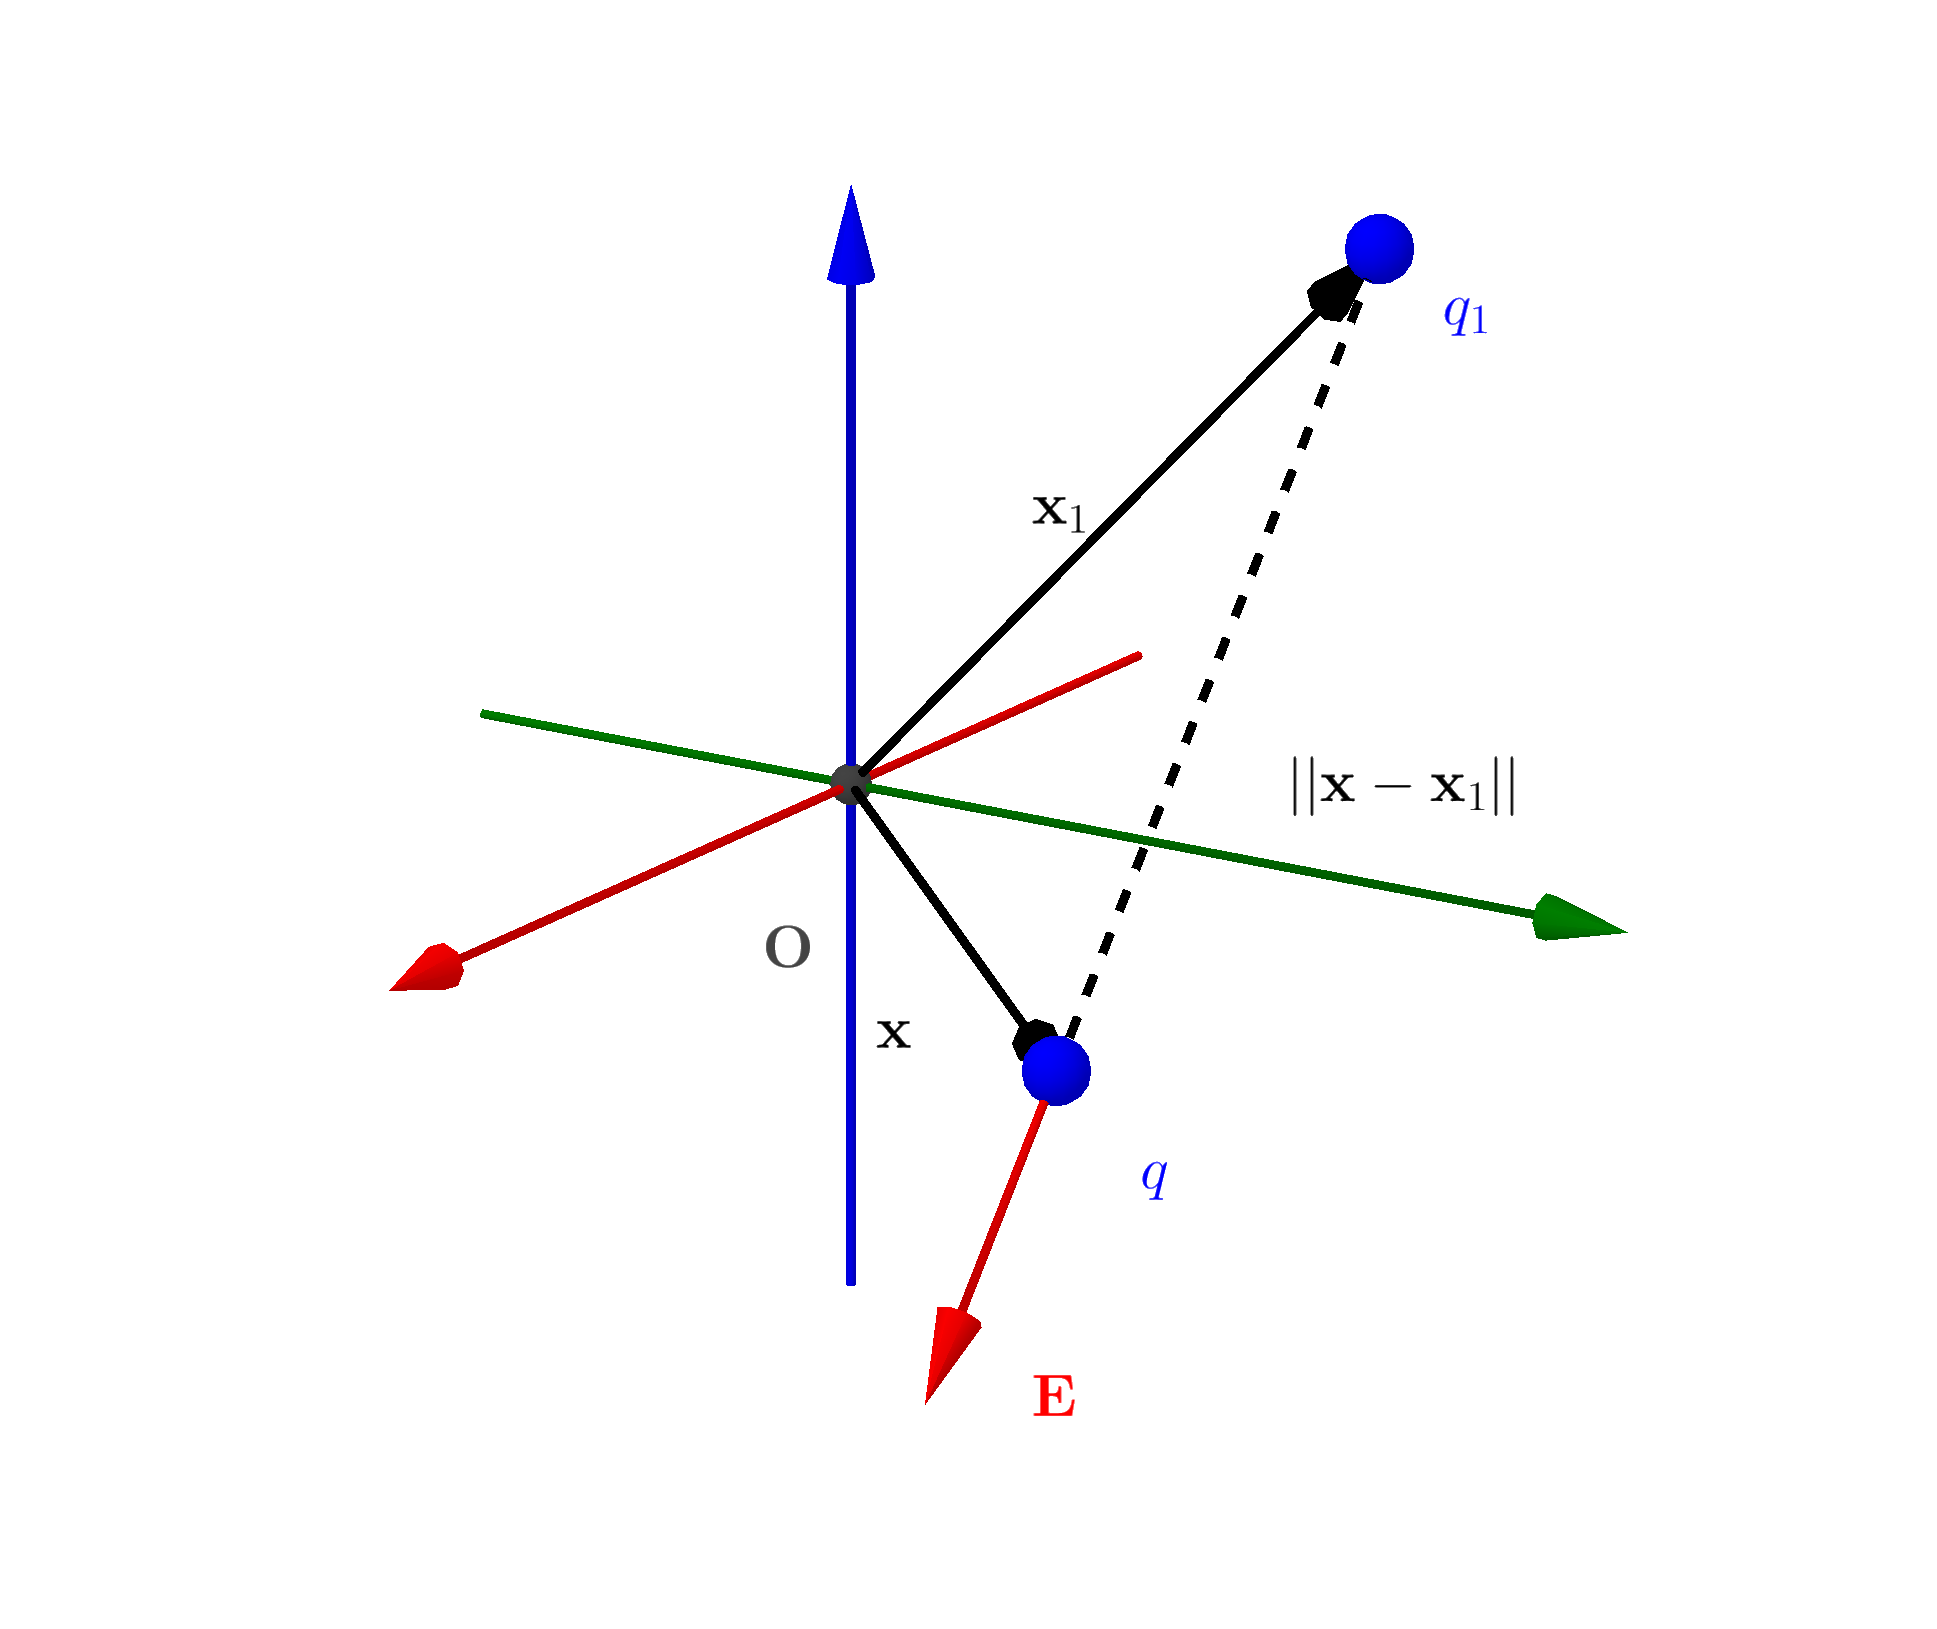
\includegraphics[scale=1]{camp_elet_3D}}
%\subfloat{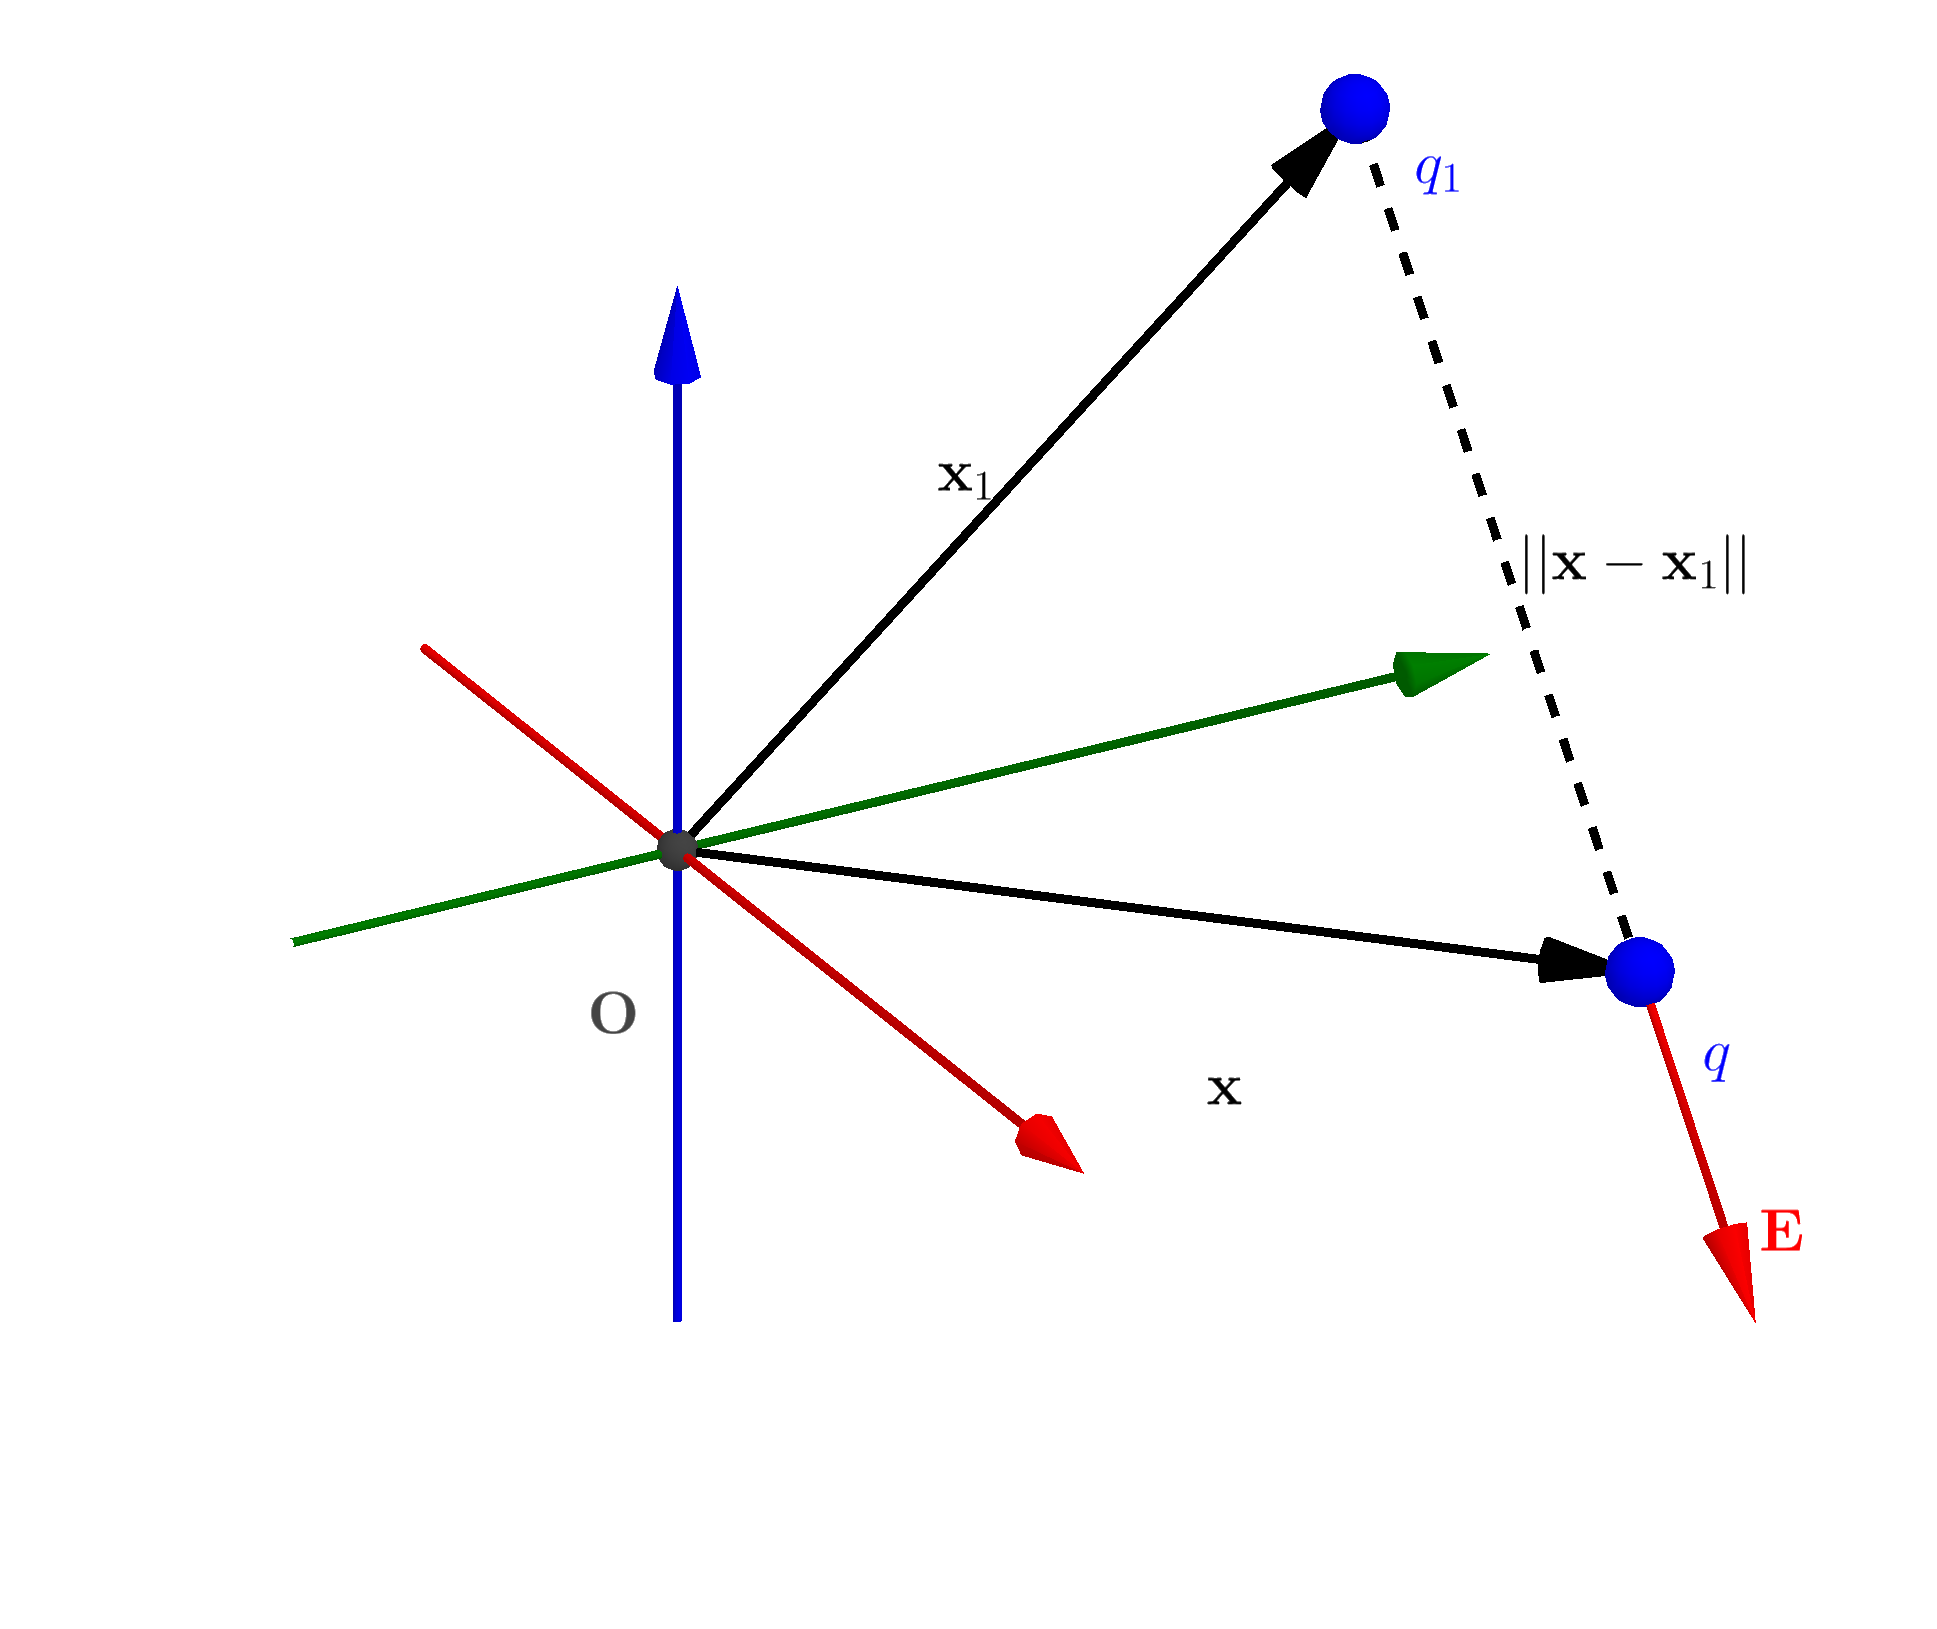
\includegraphics[scale=1]{camp_elet_3D2}}
%\caption{}
%\label{fig.mossul}
%\end{figure}

Num sistema com mais de uma carga fonte produzindo campos elétricos, foi observado experimentalmente que o campo elétrico total atuando num ponto $\textbf{x}$ é simplesmente o somatório dos campos produzidos por cada carga, o que ficou conhecido como a \textit{Superposição Linear} e pode ser expressada na forma
\begin{equation*}
\textbf{E}=k\,\sum_{i=1}^{n}q_i\,\frac{\textbf{x}_i-\textbf{x}}{||\textbf{x}_i-\textbf{x}||^3}.
\end{equation*} 
O campo elétrico devido a um pequeno número de cargas pode ser calculado a partir do princípio da superposição linear. Mas se temos uma quantidade muito grande de cargas num determinado volume $V$, devemos calcular a \textit{densidade volumétrica de carga} $\rho$ num volume infinitesimal situado em $\textbf{x}_0$ e em seguida integrar sobre o volume $V$ para obter a quantidade total de carga $Q$. A densidade de carga é definida por
\begin{equation*}
\rho(\textbf{x}_0)=\lim_{\Delta V_i \to 0}\frac{\Delta q_i}{\Delta V_i}=\frac{d\,q}{d\,V},
\end{equation*}
medida, no SI, em $C/m^3$. A quantidade total de carga $Q=\sum_i \Delta\,q_i$ no volume $V$ é
\begin{equation*}
Q=\int_{V}\rho(\textbf{x}_0)\,dV.
\end{equation*}

O \textit{fluxo elétrico} é definido como a quantidade linhas do campo elétrico que atravessam uma dada superfície, e é dado pela equação
\begin{equation*}
\Phi_\textbf{E}=\textbf{E}\cdot\textbf{A}. 
\end{equation*} 
O \textit{vetor área} é definido como a magnitude da área da superfície atravessada apontando na direção do vetor normal à superfície, $\textbf{A}=A\,\textbf{n}$, e estamos considerando um campo elétrico uniforme $\textbf{E}$ que se desloca na direção $\textbf{n}$, ou seja, é perpendicular à superfície $A$ como podemos observar na figura \ref{fig.flux_ele}.
\begin{figure}[!htb]
\centering
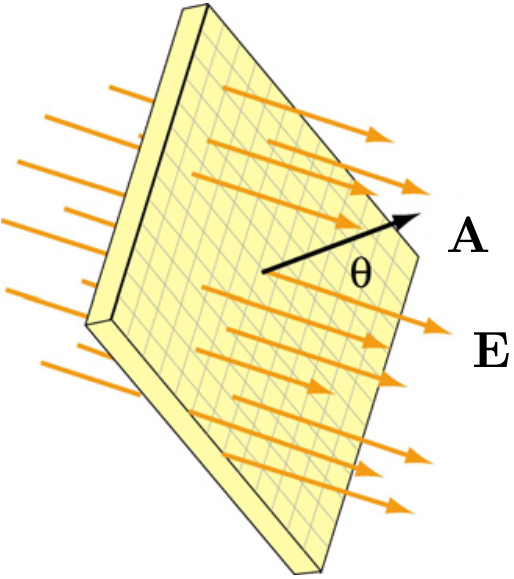
\includegraphics[scale=.5]{campo_area}
\caption{\textit{Fluxo elétrico, linhas de campo elétrico passando através de uma superfície.}}
\label{fig.flux_ele}
\end{figure}
Mas se o campo elétrico se propaga formando um ângulo $\theta$ com o vetor normal da superfície, então o fluxo elétrico é dado por
\begin{equation*}
\Phi_\textbf{E}=\textbf{E}\cdot\textbf{A}=E\,A\,\cos\theta,
\end{equation*}
com $E=\textbf{E}\cdot\textbf{n}$ sendo a componente do campo elétrico na direção $\textbf{n}$. Em geral uma superfície pode ser curva e estamos interessados numa superfície \textit{fechada}, ou seja, aquela que engloba um determinado volume, o qual contém uma carga elétrica. Tomando uma área bem pequena dessa superfície, $\Delta\textbf{A}_i$, o campo elétrico pode ser variável em cada parte da superfície e nessas condições temos que o fluxo nessa pequena região é dado por
\begin{equation*}
\Delta\,\Phi_\textbf{E}=\textbf{E}_i\cdot\Delta\,\textbf{A}_i.
\end{equation*}
O fluxo positivo atravessando toda a superfície de dentro para fora é calculado tomando o limite quando $\Delta\textbf{A}_i\to 0$ e aumentando infinitamente a quantidade dessas pequenas áreas
\begin{equation}\label{eq.fluxo_eletr}
\Phi_\textbf{E}=\lim_{i\to\infty}\sum_i\textbf{E}_i\cdot\textit{d}\textbf{A}_i=\int\int_S\textbf{E}\cdot\textit{d}\textbf{A}.
\end{equation}

Considere uma carga pontual positiva $q$ localizada no centro de uma esfera imaginária de raio $r$, onde essa carga produz um campo elétrico que aponta na direção radial conforme a figura \ref{fig.esfe_gauss}. Sabemos que a área da superfície dessa esfera é dada por $A=4\pi\,r^2$ e que, segundo a equação \ref{eq.campo_eletrico}, a magnitude do campo elétrico em qualquer ponto da superfície esférica é
\begin{equation*}
E=\frac{q}{4\pi\epsilon_0\,r^2},
\end{equation*}
assim o fluxo elétrico é calculado usando a equação \ref{eq.fluxo_eletr}.
\begin{align*}
\Phi_\textbf{E}&=\int\int_S\textbf{E}\cdot\textit{d}\textbf{A}\\
&=\int\int_S\textbf{E}\cdot\textbf{n}\,\textit{d}A\\
&=E\,\int\int_S\textit{d}A\\
&=E\,A\\
&=\frac{q}{4\pi\epsilon_0\,r^2}\,4\pi\,r^2\\
&=\frac{q}{\epsilon_0}.
\end{align*}
Na demonstração acima escolhemos uma esfera como \textit{superfície Gaussiana} mas, introduzindo o conceito de \textit{ângulo sólido}, vemos que a demonstração é válida para qualquer superfície fechada, utilizada em aplicações que apresentem mais ou menos alguma simetria (esférica, planar ou cilíndrica). Para mais detalhes consultar \cite{jackson_classical_1999}. Assim, concluímos que o fluxo elétrico através de uma superfície fechada que apresente mais ou menos alguma simetria é diretamente proporcional à quantidade de carga enclausurada pela superfície. Matematicamente, a \textit{lei de Gauss} para o fluxo elétrico é
\begin{equation*}
\Phi_\textbf{E}=\int\int_S\textbf{E}\cdot\textit{d}\textbf{A}=\frac{q}{\epsilon_0}.
\end{equation*}
\begin{figure}[!htb]
\centering
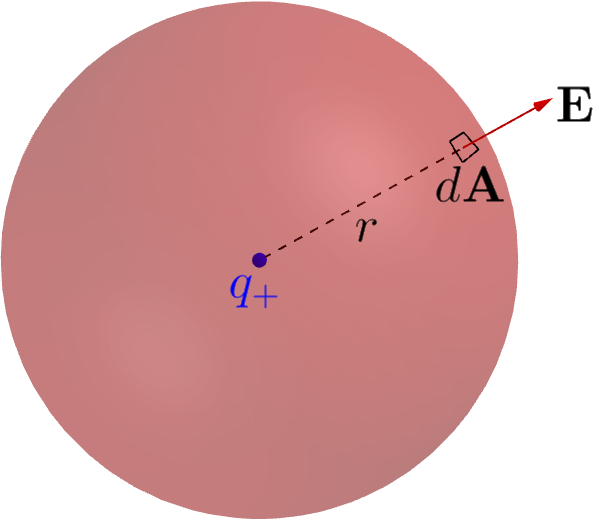
\includegraphics[scale=.3]{esfera_gaussiana}
\caption{\textit{Esfera Gaussiana enclausurando uma carga positiva $q$. Nessas condições, o ângulo entre o vetor campo elétrico e o vetor normal à superfície infinitesimal $d\textbf{A}$ é zero.}}
\label{fig.esfe_gauss}
\end{figure}

Uma carga elétrica produz um campo elétrico, e de maneira similar uma barra magnética, ou ímã, produz um \textit{campo magnético} $\textbf{B}$. Um ímã possui um polo norte de onde partem as linhas de campo magnético e um polo sul por onde as linhas de campo magnético retornam ao ímã (figura \ref{fig.barras_mag}). Diferentemente das cargas elétricas que são observadas isoldamente na natureza, os dois polos magnéticos sempre aparecem aos pares, ou seja, monopolos magnéticos não existem isoladamente apesar de a suposição de sua existência ser de interesse teórico. Assim, sempre que um ímã é fracionado, mesmo que em partes muito elementares, o resultado sempre será um novo ímã com dois polos magnéticos conforme a figura \ref{fig.barras_mag}.
\begin{figure}[!htb]
\centering
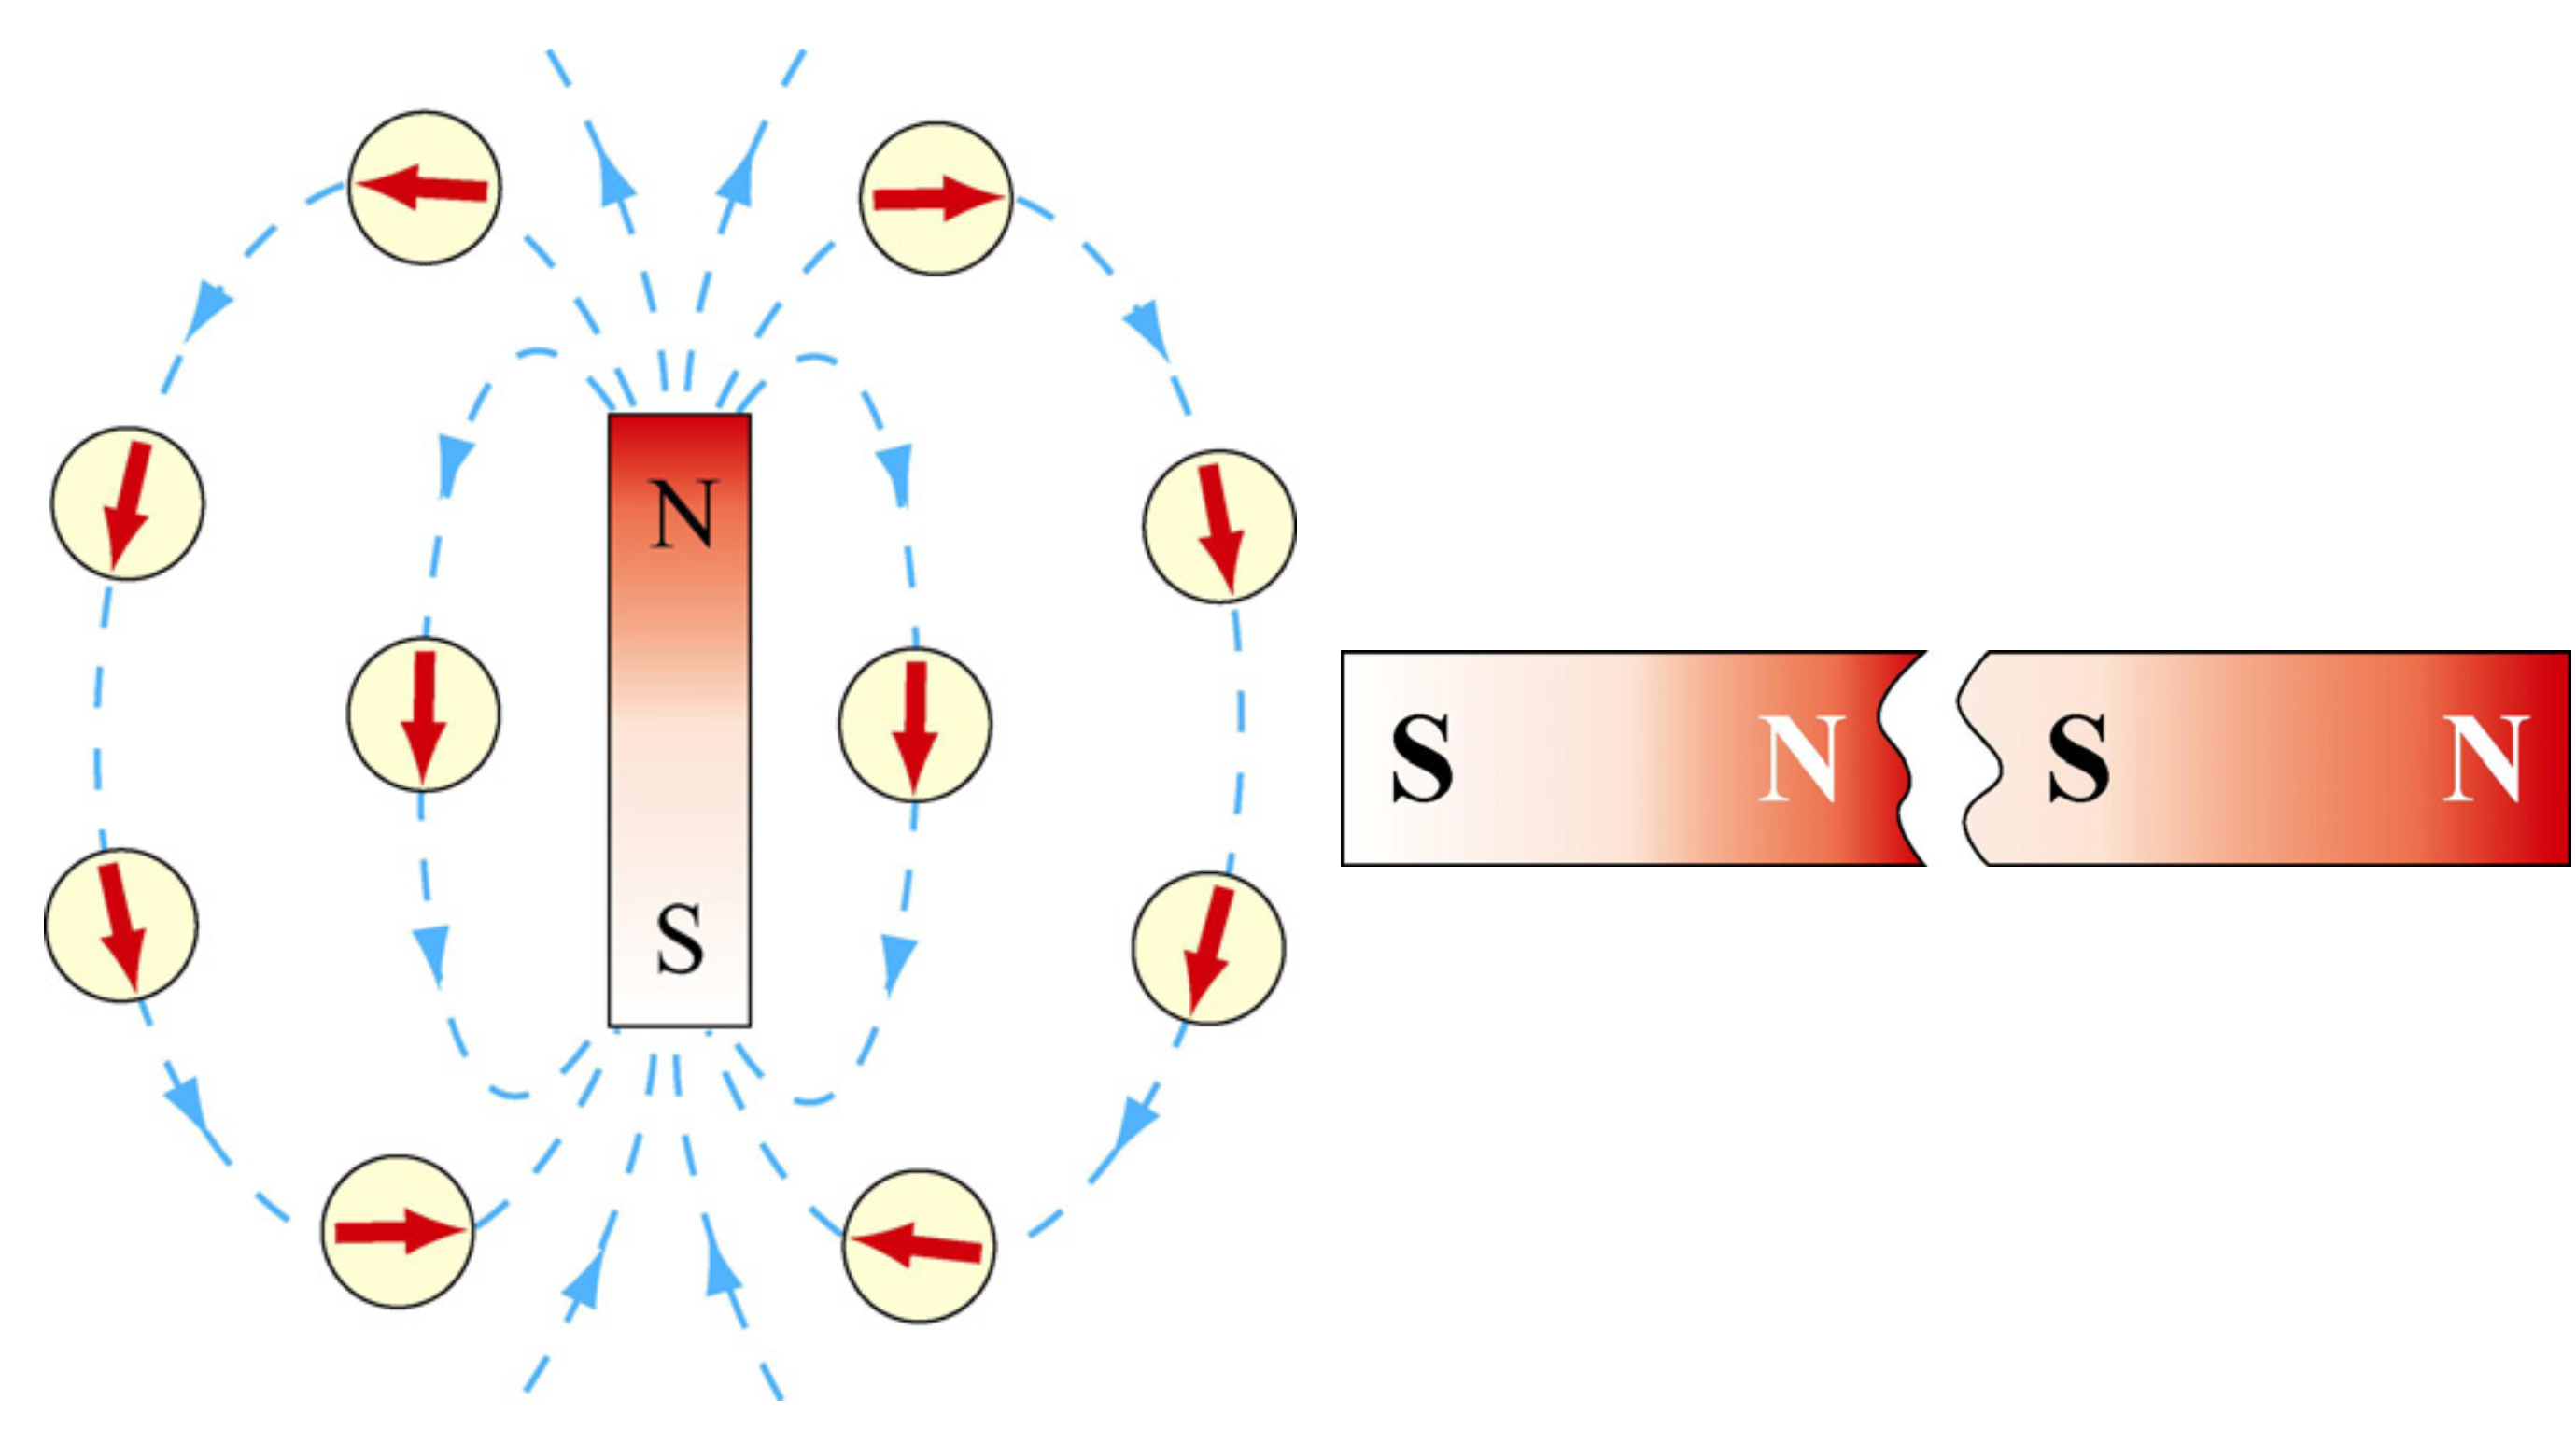
\includegraphics[scale=.7]{barras_magn}
\caption{\textit{Barras magnéticas onde polos de mesmo sinal se repelem e polos de sinais contrários se atraem.}}
\label{fig.barras_mag}
\end{figure}
Como não existem monopolos magnéticos, o campo magnético deve ser definido de forma diferente do campo elétrico, e experimentalmente foram observadas algumas características relacionadas ao movimento de uma carga elétrica $q$ com velocidade $\textbf{v}$ num campo magnético $\textbf{B}$:
\begin{itemize}
\item a magnitude da força magnética $\textbf{F}_B$ é proporcional à $v$, $B$ e $q$, onde $v$ e $B$ são as magnitudes da velocidade e do campo magnético respectivamente,
\item a direção de $\textbf{F}_B$ é perpendicular ao plano formado por $\textbf{v}$ e $\textbf{B}$,
\item $\textbf{F}_B$ é proporcional ao $\sin\theta$, o ângulo formado por $\textbf{v}$ e $\textbf{B}$. Se $\textbf{v}$ e $\textbf{B}$ são paralelos então $\textbf{F}_B=0$, e
\item o sentido de $\textbf{F}_B$ depende do sinal da carga $q$.
\end{itemize}
Essas observações são ilustradas na figura \ref{fig.froca_mag_veloc} e a força magnética é definida como
\begin{equation*}
\textbf{F}_B=q\textbf{v}\times\textbf{B}.
\end{equation*}
\begin{figure}[!htb]
\centering
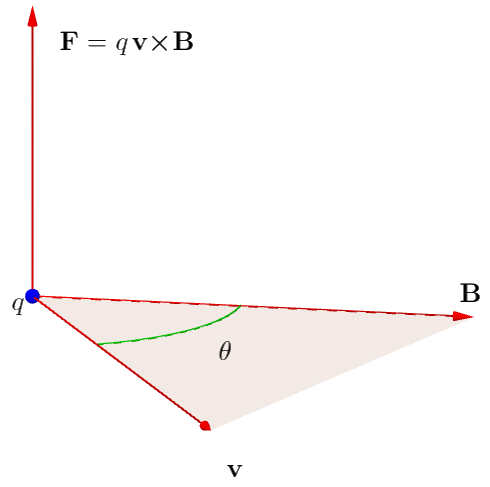
\includegraphics[scale=.4]{forca_camp_mag_veloc}
\caption{\textit{Força magnética agindo numa carga elétrica que se desloca num campo magnético.}}
\label{fig.froca_mag_veloc}
\end{figure}
Teoricamente, poderíamos tentar determinar a lei de Gauss para o fluxo magnético com o mesmo procedimento aplicado ao fluxo elétrico e obter
\begin{equation*}
\Phi_\textbf{B}=\int\int_S\textbf{B}\cdot\textit{d}\textbf{A}=\frac{q_m}{\mu_0},
\end{equation*} 
onde $q_m$ é a carga magnética (suposto monopolo magnético) enclausurado pela superfície Gaussiana, $B$ é o campo magnético e $\mu_0$ é a \textit{permeabilidade magnética no vácuo} com valor $\mu_0=4\,\pi\times 10^{-7} T.m/A$. No entanto, não foi constatada a existência de qualquer carga magnética isolada mesmo após muitos esforços. Como $q_m=0$, temos que a lei de Gauss para o magnetismo é
\begin{equation}\label{eq.gauss_flux_mag}
\Phi_\textbf{B}=\int\int_S\textbf{B}\cdot\textit{d}\textbf{A}=0.
\end{equation}
Conforme podemos ver na figura tal, a equação \ref{eq.gauss_flux_mag} implica que a quantidade de linhas do campo magnético saindo da superfície é igual à quantidade que está entrando, ou seja, não há uma origem isolada e um término isolado para o fluxo magnético como há para o fluxo elétrico. Outro problema é que a barra imantada atravessa a superfície que, de acordo com a hipóteses da lei de Gauss, deveria ser fechada.
\begin{figure}[!htb]
\centering
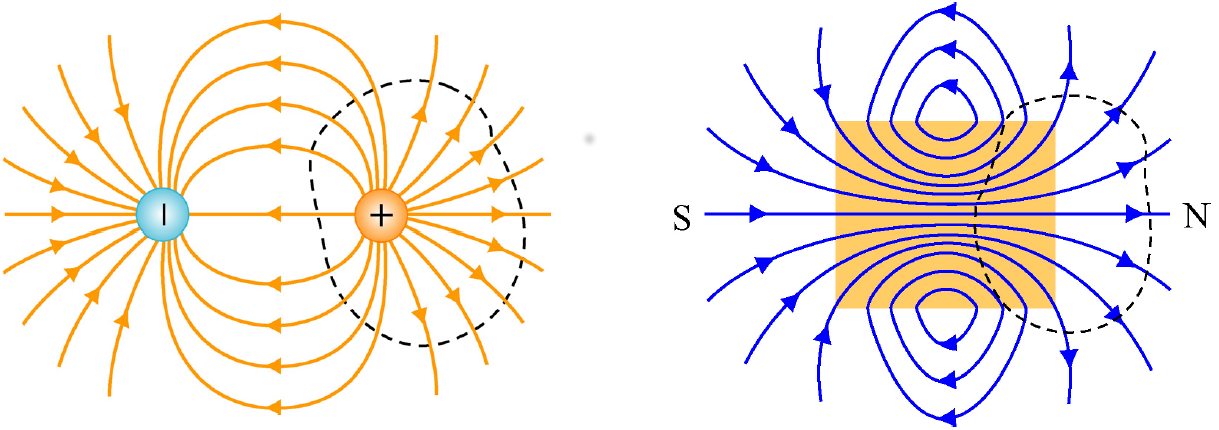
\includegraphics[scale=.3]{flux_ele_mag}
\caption{\textit{As linhas do campo magnético que emanam do polo norte do ímã em direção ao polo sul retornam para dentro da superfície Gaussiana descrevendo um laço fechado.}}
\label{fig.flux_elet_magn}
\end{figure}

\subsection{A Lei de Ampère}
Correntes elétricas podem ser produzidas por cargas elétricas que se movem num fio condutor. Essas correntes elétricas são fontes de campos magnéticos $d\,\textbf{B}$, num determinado ponto $x$, e que podem ser calculados em função da corrente $I$ num intervalo infinitesimal $d\,\textbf{l}$ do fio. Visualização na figura \ref{fig.corrente_fio}. A fonte de corrente infinitesimal é dada por $I\,d\,\textbf{l}$ e $r$ é a distância entre o ponto de aplicação do campo magnético e a fonte de corrente infinitesimal. O vetor $\textbf{n}$ é o vetor normal que aponta na direção de $x$ e o vetor $d\,\textbf{l}$ aponta na direção e sentido da corrente $I$. 
\begin{figure}
\centering
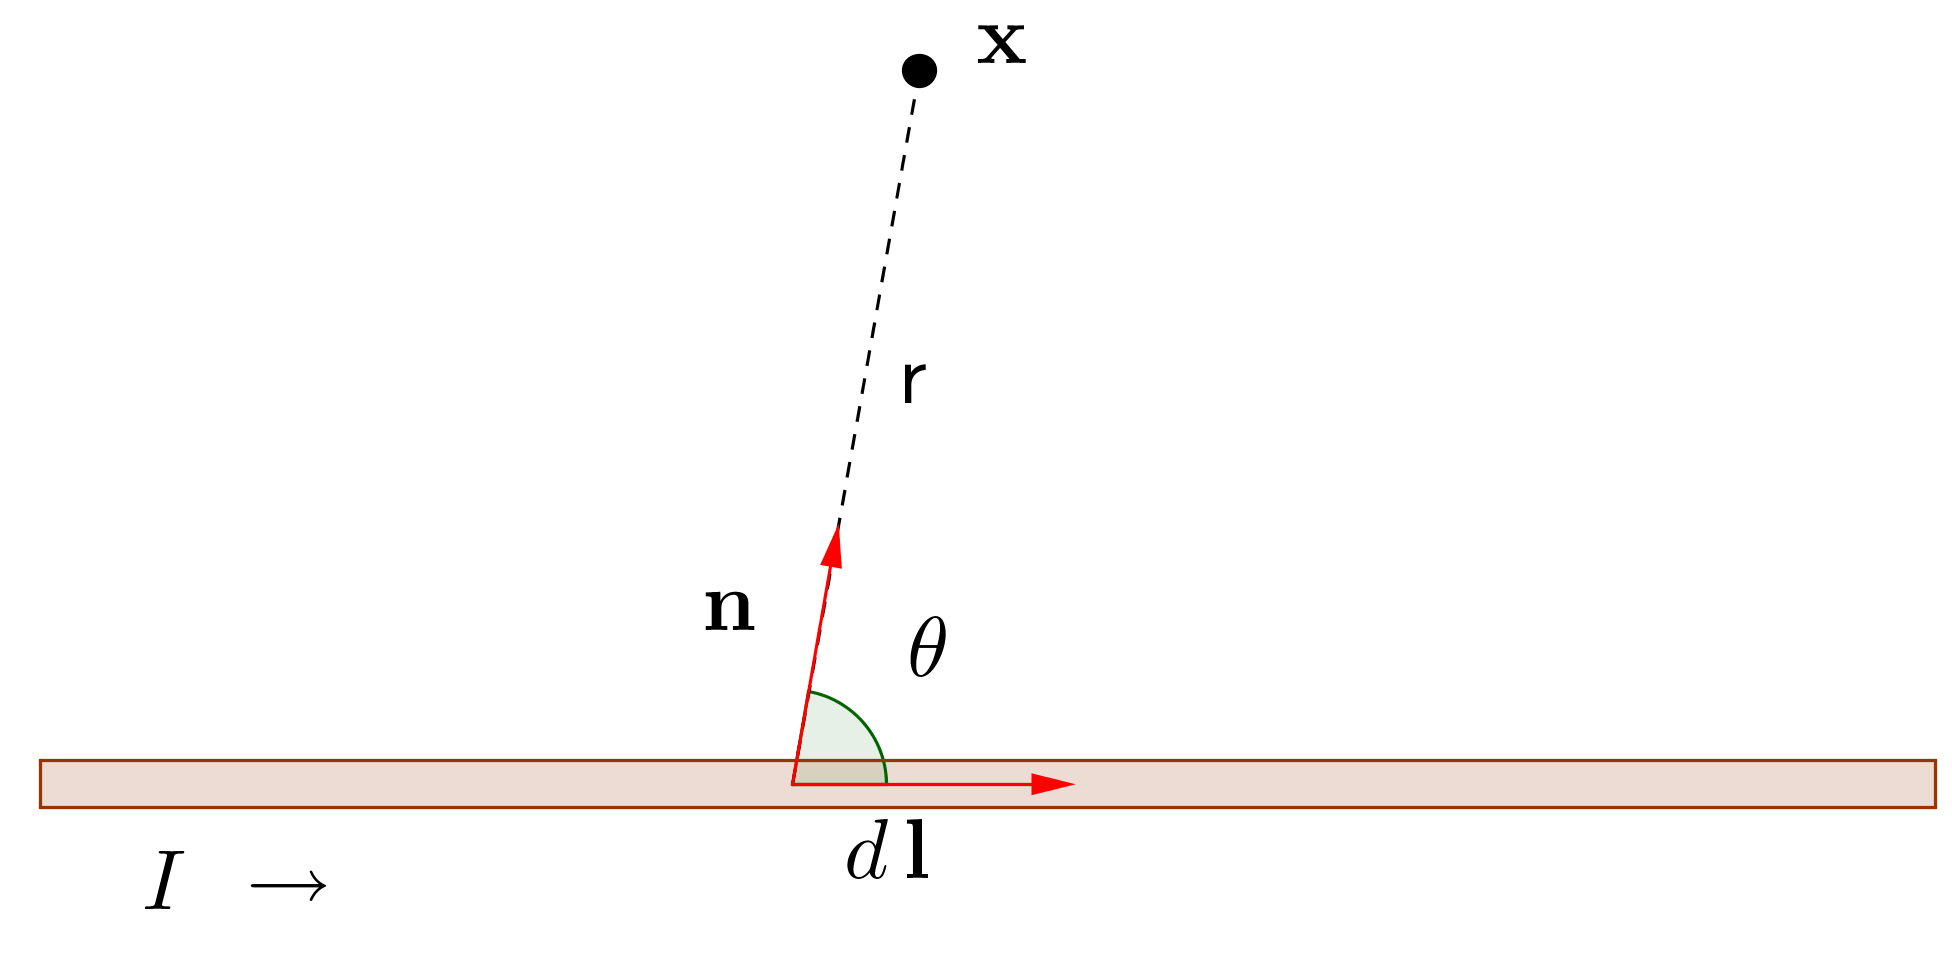
\includegraphics[scale=1.1]{corrente_fio}
\caption{\textit{Campo magnético no ponto $\textbf{x}$ devido a passagem de uma corrente elétrica $I$ pelo fio. Observe que a magnitude do campo depende também do ângulo $\theta$ entre $\textbf{l}$ e $\textbf{n}$}.}
\label{fig.corrente_fio}
\end{figure}
Assim sendo, a \textit{Lei de Biot-Savart} tem definição análoga à lei de Coulomb e pode ser expressa como
\begin{equation}\label{eq.lei_biot_savart}
d\,\textbf{B}=\frac{\mu_0\,I}{4\,\pi}\frac{d(\textbf{l}\times\textbf{n})}{r^2},
\end{equation}
e o campo magnético no volume ao redor do fio pode ser obtido integrando sobre a direção perpendicular ao plano formado por $\textbf{l}$ e $\textbf{n}$ ao longo do comprimento do fio.
\begin{equation}
\textbf{B}=\frac{\mu_0I}{4\,\pi}\int_{\textbf{l}}\frac{d(\textbf{l}\times\textbf{n})}{r^2}.
\end{equation}

Considere agora um laço circular (linha de campo magnético) de raio $r$ contido num plano perpendicular ao fio condutor, divido em pequenos comprimentos $\Delta\textbf{s}=\Delta s\,\pmb{\phi}$, cujos vetores correspondentes apontam na direção do vetor tangencial à circunferência naquele ponto, conforme  a figura tal. Esse laço fechado contido num plano é denominado \textit{laço Amperiano} e é usado para calcular o campo magnético referente àquela linha de campo tomando o limite quando $\Delta\textbf{s}\to 0$ e integrando no intervalo dado pelo comprimento da circunferência. Repare, pela figura \ref{fig.corrente_fio}, que nesse caso $\theta=\pi rd$ e que $\pmb{\phi}$ é perpendicular ao plano formado por $\textbf{l}$ e $\textbf{n}$, portanto a magnitute do vetor  $\textbf{B}$ na direção $\pmb{\phi}$ é dada pela lei de Biot-Savart na equação \ref{eq.lei_biot_savart}.
\begin{equation*}
\int_{s}\textbf{B}\cdot d\textbf{s}=B\int_{s}ds=\frac{\mu_0I}{2\pi\,r}2\pi\,r=\mu_0I.
\end{equation*} 
\begin{figure}[h]
\centering
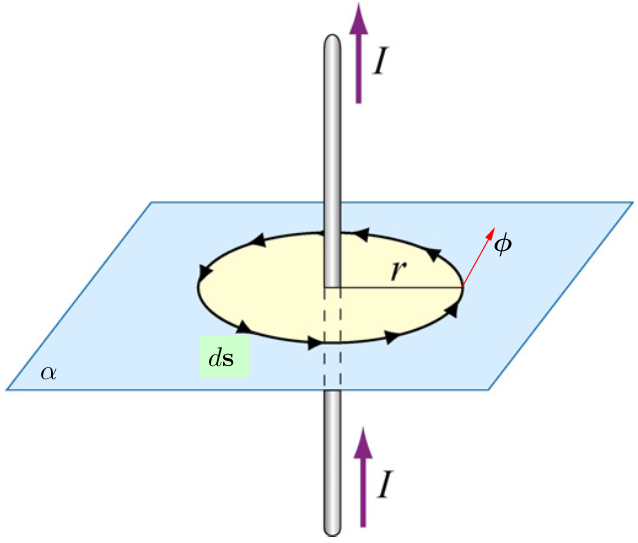
\includegraphics[scale=.5]{laco_amperiano}
\caption{\textit{Laço amperiano seguindo a regra da mão direita: posicionando o polegar no sentido da corrente, o campo magnético tem o mesmo sentido dos demais dedos curvando em torno do fio.}}
\label{fig.laco_amperiano}
\end{figure}

Vamos considerar um outro exemplo de laço amperiano cujo contorno denotado por $abcda$ se sobrepõe a duas linhas de campo magnético coplanares, observado na figura tal. No desenvolvimento abaixo, a primeira e terceira integrais zeram pois o campo magnético é perpendicular ao caminho de integração nesses intervalos, e $B_2(r_2\theta)$ e $B_1[r_1(2\pi-\theta)]$ são os comprimentos dos arcos $bc$ e $da$, respectivamente. A integral de linha do campo magnético no contorno $abcda$ é
\begin{align*}
\int_{abcda}\textbf{B}\cdot d\textbf{s}&=\int_{ab}\textbf{B}\cdot d\textbf{s}+\int_{bc}\textbf{B}\cdot d\textbf{s}+\int_{cd}\textbf{B}\cdot d\textbf{s}=\int_{da}\textbf{B}\cdot d\textbf{s}\\
&=0+B_2(r_2\theta)+0+B_1[r_1(2\pi-\theta)]\\
&=\frac{\mu_0I}{2\pi\,r_2}(r_2\theta)+\frac{\mu_0I}{2\pi\,r_1}[r_1(2\pi-\theta)]\\
&=\frac{\mu_0I}{2\pi}\theta+\frac{\mu_0I}{2\pi}(2\pi-\theta)\\
&=\mu_0I.
\end{align*}
\begin{figure}
\centering
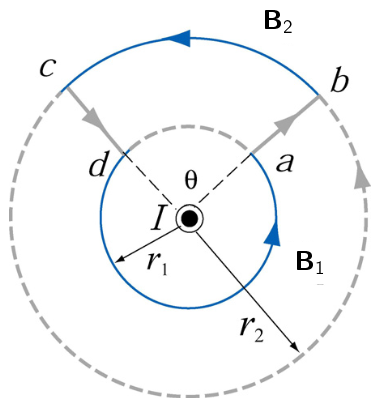
\includegraphics[scale=.5]{laco_amperiano_2}
\caption{\textit{Laço amperiano passando por duas linhas de campo. O ponto no centro significa que o sentido da corrente elétrica está ``saindo do plano do papel".}}
\label{fig.laco_amper_2}
\end{figure}
Vemos o mesmo resultado se o laço amperiano envolve uma ou duas linhas de campo magnético e, usando coordenadas cilíndricas, podemos demonstrar que o mesmo resultado é válido para uma quantidade arbitrária de linhas de campo magnético, ou seja, a integral de linha do campo magnético através de qualquer laço amperiano fechado é proporcional à corrente elétrica inscrita no laço. A \textit{Lei de Ampère} é dada por
\begin{equation*}
\int_{s}\textbf{B}\cdot d\textbf{s}=\mu_0I.
\end{equation*}
Analogamente à lei de Gauss para campos elétricos, para ser aplicada a lei de Ampère é necessário que o laço possua alguma simetria em relação ao fio. No caso de um fio condutor suficientemente grande para que suas extremidades não interfiram na aplicação, temos uma simetria cilíndrica e a lei de Ampère pode ser aplicada normalmente. Caso contrário, devemos utilizar a lei de Biot-Savart. 

Agora considere a seguinte situação, descrita por Maxwell, onde o circuito elétrico está interrompido por um capacitor. 
\begin{figure}
\centering
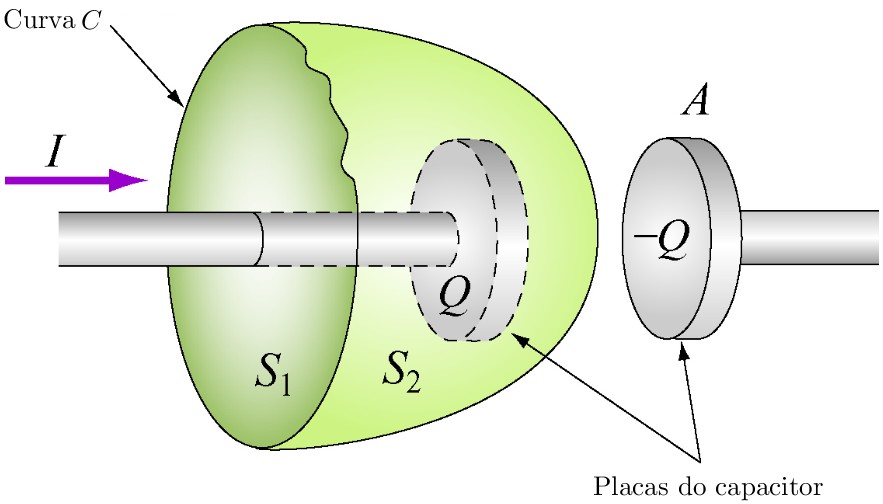
\includegraphics[scale=.3]{capacitor}
\caption{\textit{Quando há corrente no circuito, cargas positivas se acumulam numa placa do capacitor assim como cargas negativas se acumulam na outra placa. Tal acúmulo gera um fluxo elétrico variável entre as placas.}}
\label{fig.capacitor}
\end{figure}
Como vimos pela lei de Ampère, o campo magnético depende somente da corrente no circuito e do comprimento da circunferência que limita a superfície atravessada pelo fio condutor, e não depende dessa superfície em si. Portanto, o campo magnético referente à curva $C$ da figura \ref{fig.capacitor} pode ser calculado considerando a superfície $S_1$ ou a superfície $S_2$. A superfície $S_1$ é atravessada pela corrente $I$ a qual produz o campo magnético $\mathbf{B}$, mas superfície $S_2$ não é atravessada por $I$ e, no entanto, é produzido o mesmo campo magnético $\mathbf{B}$. Assim podemos sugerir que exista um outro fenômeno físico entre as placas do capacitor que seja responsável pela geração de $\mathbf{B}$. À medida que o capacitor vai sendo carregado, cargas elétricas opostas vão se acumulando em sua placas gerando um campo elétrico variável entre as placas, o qual produz um fluxo elétrico variável através da área da placa do capacitor. Maxwell mostrou que que o produto da variação desse fluxo elétrico pela permissividade elétrica no vácuo era numericamente igual à corrente $I$, e por isso produzia o mesmo campo $\mathbf{B}$ quando integrado longo da curva $C$,
\begin{equation*}
I_d=\epsilon_0\frac{d\phi_E}{dt}.
\end{equation*}
Tal produto foi denominado \textit{corrente deslocada} e foi adicionado à lei de Ampère, a qual se tornou a \textit{lei de Ampére generalizada} ou \textit{lei de Ampère-Maxwell},
\begin{equation*}
\int_s\mathbf{B}\cdot d\mathbf{s}=\mu_0I+\mu_0\epsilon_0\frac{d\phi_E}{dt}.
\end{equation*}
Note que quando consideramos a superfície $S_1$, $I_d=0$ já que o fluxo elétrico é constante e assim $\mathbf{B}$ é dado somente por $I$. Quando consideramos a superfície $S_2$, $I=0$ e $\mathbf{B}$ é dado somente por $I_d$. 




\subsection{A Lei de Faraday}
Analogamente ao caso da força gravitacional, o \textit{trabalho} $W$ realizado por uma força elétrica $\textbf{F}_e$ para levar uma carga elétrica $q$ de um ponto $A$ até um ponto $B$ é definido como
\begin{equation}\label{eq.trabalho}
W=\int_{A}^{B}\textbf{F}_e\cdot d\textbf{s}.
\end{equation}
A diferença entre a \textit{energia potencial} $U$ em cada um dos pontos $A$ e $B$ é o que ocasiona o deslocamento da carga, assim a variação da energia potencial tem definição
\begin{equation}\label{eq.energia_potencial}
\Delta U=U_b-U_a=-\int_{A}^{B}\textbf{F}_e\cdot d\textbf{s}=-W.
\end{equation}
A \textit{diferença de potencial elétrico}, $\Delta V$, também chamada \textit{ddp}, é variação da energia potencial por unidade de carga elétrica $q$. Utilizando a equação \ref{eq.camp_elet}, que relaciona força elétrica e campo elétrico, podemos definir a ddp como
\begin{equation}\label{eq.ddp}
\Delta V=-\int_{A}^{B}\frac{\textbf{F}_e}{q}\cdot d\textbf{s}=-\int_{A}^{B}\textbf{E}\cdot d\textbf{s}
\end{equation}
A ddp representa a quantidade de trabalho por unidade de carga para mover a carga do ponto $A$ ao ponto $B$ e sua unidade de medida no SI é o volt ($V=\frac{J}{C}$). Observe nas definições acima que só importa os valores no pontos $A$ e $B$, e não importa necessariamente o caminho que a carga vai percorrer de um ponto até o outro. 

Agora, num circuito elétrico fechado, as cargas percorrem um determinado caminho a partir de uma fonte de energia elétrica. Essa fonte é chamada de \textit{força eletromotriz}, representada por $\varepsilon$, e que pode ser pensada como uma ``bomba" de cargas que as impulsiona de um potencial menor para um potencial maior. A força eletromotriz é definida como o trabalho realizado para mover uma carga unitária na direção de maior potencial, matematicamente,
\begin{equation*}
\varepsilon=\frac{dW}{dq}, 
\end{equation*}
também medida em volt. Como o campo magnético não produz trabalho, o trabalho realizado sobre o movimento das cargas deve ser devido a um campo elétrico e para escrever a força eletromotriz em termos do campo elétrico de forma análoga ao que foi feito nas equações \ref{eq.trabalho}, \ref{eq.energia_potencial} e \ref{eq.ddp}, devemos utilizar uma integral de linha, pois nesse caso a corrente percorre um determinado caminho. Como o campo elétrico é não-conservativo (senão não haveria corrente) o valor da integral é diferente de zero. Assim,
\begin{equation}\label{eq.emf_E_nc}
\varepsilon=\int_{linha}\pmb{E}\cdot d\pmb{s}.
\end{equation}
 
O \textit{fluxo magnético} é definido de maneira similar ao fluxo elétrico e o entendimento pode ser acompanhado pela figura \ref{fig.flux_ele}. O fluxo magnético através de uma superfície é definido como
\begin{equation*}
\phi_B=\textbf{B}\textbf{A}=B\,A\,\cos\theta,
\end{equation*}
onde o vetor área é $\textbf{A}=A\textbf{n}$, $\textbf{n}$ é o vetor normal à superfície atravessada, $A$ é a magnitude da área, $B=\textbf{B}\cdot\textbf{n}$ é a componente do campo magnético na direção do vetor normal e $\theta$ é o ângulo entre $\textbf{B}$ e $\pmb{A}$. Tomando um elemento infinitesimal da área e integrando sobre a superfície o fluxo magnético é
\begin{equation*}
\phi_B=\int\int_S\pmb{B}\,d\pmb{A},
\end{equation*}
medido em \textit{Weber}, $Wb=\frac{T}{m^2}$. 

Em 1831, Faraday descobriu que se pode criar um campo elétrico variando um campo magnético em função do tempo num fenômeno que foi batizado de \textit{indução eletromagnética}. Um dos experimentos de Faraday (figura tal) consiste em movimentar um ímã dentro de uma bobina feita de fio condutor onde se pode observar a geração de uma corrente elétrica, como se a bobina estivesse conectada a fonte de força eletromotriz. O experimento mostra que a força eletromotriz induzida é proporcional à taxa (negativa) de variação do fluxo magnético através da bobina, a \textit{lei de Faraday} é
\begin{equation*}
\varepsilon=-\frac{d\phi_B}{dt}.
\end{equation*}
Podemos reescrever a lei de Faraday usando a equação \ref{eq.emf_E_nc},
\begin{equation*}
\varepsilon=\int_{linha}\pmb{E}\cdot d\pmb{s}=-\frac{d\phi_B}{dt},
\end{equation*}
o que implica que a variação do fluxo magnético induz um campo elétrico não-conservativo que varia com o tempo, diferente do campo elétrico conservativo gerado por cargas elétricas estacionárias.

%\begin{figure}[!htb]
%\centering
%\includegraphics[scale=5]{•}
%\caption{\textit{•}}
%\label{fig.exper_faraday}
%\end{figure}









\section{Equações de Maxwell}

\section{Generalizações da teoria}

\section{Conclusões}
\chapter{Fundamentos de Elasticidade}\label{sec.fund_elast}

\section{Introdu\c{c}\~ao}
A teoria formal da propaga\c{c}\~ao de ondas s\'ismicas repousa nas intera\c{c}\~oes entre as part\'iculas infinitesimais discretas do meio \`a medida que uma deforma\c{c}\~ao se propaga. \'E muito dif\'icil estudar individualmente cada uma dessas intera\c{c}\~oes, mas dados experimentais que foram coletados como resultados dessas intera\c{c}\~oes sugerem que as mesmas podem ser consideradas em conjunto. Assim, o estudo da propaga\c{c}\~ao de ondas s\'ismicas atrav\'es de camadas de subsuperf\'icie num material discretizado pode ser feito considerando o meio como cont\'inuo, e tais estudos s\~ao os objetos da \textit{mec\^anica do cont\'inuo}. 

No desenvolvimento te\'orico da mec\^anica do cont\'inuo n\~ao s\~ao consideradas as caracter\'isticas at\^omicas da mat\'eria bem como as intera\c{c}\~oes entre essas part\'iculas, ou seja, a mat\'eria n\~ao \'e estudada do ponto de vista microsc\'opico. Segundo \cite{slawinski}, tal abordagem se justifica pelo fato de que a mat\'eria \'e formada por part\'iculas suficientemente pouco espa\c{c}adas e suas caracter\'isticas e comportamento podem ser descritos por fun\c{c}\~oes cont\'inuas e diferenci\'aveis. Assim, \'e assummido que elementos infinitesimais da mat\'eria t\^em as mesmas propriedades observadas em experimentos macrosc\'opicos, pois essa hip\'otese permite a cria\c{c}\~ao de um modelo matem\'atico abstrato \textit{efetivo} na descri\c{c}\~ao da realidade f\'isica. Como exemplo, vamos considerar a cor de um objeto. Pr\'otons e el\'etrons n\~ao possuem cor, mas os meios materiais (que s\~ao formados por pr\'otons e el\'etrons) t\^em a capacidade de absorver ou refletir determinados comprimentos de ondas eletromagn\'eticas as quais determinam a cor de cada meio. Outros conceitos da mec\^anica do cont\'inuo s\~ao elasticidade, viscosidade, fric\c{c}\~ao, rigidez, etc, como veremos mais a frente.


\section{Fatos experimentais}
A teoria sobre elasticidade est\'a baseada em conceitos primitivos e conclus\~oes estabelecidas a partir de fatos experimentais verificados em v\'arios textos sobre o assunto como \cite{liu}, \cite{dahlem} e \cite{slawinski}. Adicionalmente, em geral as equa\c{c}\~oes que governam a propaga\c{c}\~ao de ondas em meios el\'asticos s\~ao n\~ao-lineares. Contudo, em experimentos s\'ismicos foi constatado que aspectos importantes da propaga\c{c}\~ao de ondas podem ser analisados a partir de equa\c{c}\~oes lineares, resultando numa abordagem chamada \textit{teoria da elasticidade linearizada}.

\subsection{Deforma\c{c}\~ao}

A \textit{deforma\c{c}\~ao} de um meio el\'astico cont\'inuo \'e a mudan\c{c}a na posi\c{c}\~ao dos pontos que comp\~oem o corpo em rela\c{c}\~ao uns aos outros. Ou seja, h\'a uma mudan\c{c}a relativa entre os pontos e n\~ao um deslocamento do corpo como um todo e sem mudan\c{c}a de sua forma, caso em que ter\'iamos um \textit{movimento r\'igido}. Nesta subse\c{c}\~ao estamos interessados nas caracter\'isticas geom\'etricas relativas \`a deforma\c{c}\~ao de um corpo. N\~ao estamos considerando as causas de deforma\c{c}\~ao de um corpo, como aplica\c{c}\~ao de carga ou varia\c{c}\~ao de temperatura, nem discutiremos a composi\c{c}\~ao do material, assumindo apenas que o mesmo seja cont\'inuo e el\'astico. Assim, vamos relacionar as caracter\'isticas geom\'etricas de um corpo antes da deforma\c{c}\~ao com as caracter\'isticas ap\'os a deforma\c{c}\~ao.

\subsection{Dedu\c{c}\~ao do Tensor de Deforma\c{c}\~oes}\label{sec.deriva_deforma}

Para determinar o tensor de deforma\c{c}\~oes vamos considerar dois pontos pertencentes ao espaco $\mathbb{R}^3$ bastante pr\'oximos um do outro denotados por
\begin{align*}
\mathbf{x}&=(x_1,x_2,x_3)\quad\text{e}\\
\mathbf{y}=\mathbf{x}+d\mathbf{s}&=(x_1+dx_1,x_2+dx_2,x_3+dx_3),
\end{align*}
e que podem ser observados na figura \ref{fig.deformacao_meio}. O quadrado da dist\^ancia entre esses dois pontos \'e
\begin{equation}\label{eq.dist_antes_defor}
\norm{d\mathbf{s}}^2=(dx_1)^2+(dx_2)^2+(dx_3)^2.
\end{equation}
\begin{figure}
\centering
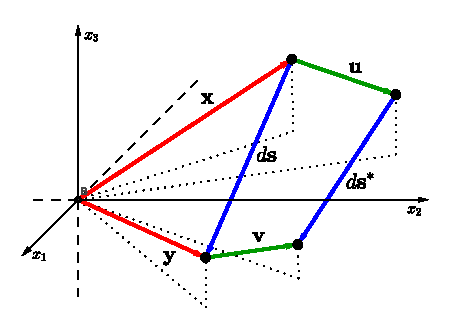
\includegraphics[scale=1.4]{deformacao_meio}
\caption{\textit{Mudan\c{c}a na posi\c{c}\~ao relativa entre os pontos que comp\~oem um  meio el\'astico cont\'inuo.}}
\label{fig.deformacao_meio}
\end{figure}
A aplica\c{c}\~ao de uma deforma\c{c}\~ao depende do ponto de aplica\c{c}\~ao, ou seja, a deforma\c{c}\~ao aplicada no ponto $\mathbf{x}$ difere da aplica\c{c}\~ao no ponto $\mathbf{y}$. Caso o vetor que d\'a a deforma\c{c}\~ao tenha componentes constantes, n\~ao teremos uma deforma\c{c}\~ao relativa, apenas uma transla\c{c}\~ao dos pontos. Assim, podemos definir o \textit{vetor de deslocamento} para cada ponto de aplica\c{c}\~ao
\begin{align*}
\mathbf{u}(\mathbf{x})&=(u_1,u_2,u_3),\\
\mathbf{v}(\mathbf{y})&=(v_1,v_2,v_3),
\end{align*}
e som\'a-los aos respectivos pontos $\mathbf{x}$ e $\mathbf{y}$ para obter suas posi\c{c}\~oes ap\'os a deforma\c{c}\~ao,
\begin{align*}
\mathbf{x}^*&=(x_1+u_1,x_2+u_2,x_3+u_3)\\
\mathbf{y}^*&=(x_1+dx_1+v_1,x_2+dx_2+v_2,x_3+dx_3+v_3).
\end{align*}
Subtraindo, obtemos o vetor que d\'a a diferen\c{c}a entre os pontos ap\'os a deforma\c{c}\~ao
\begin{equation}\label{eq.dist_apos_defor}
d\mathbf{s}^*=(dx_1+v_1-u_1,dx_2+v_2-u_2,dx_3+v_3-u_3).
\end{equation}
Como a varia\c{c}\~ao entre os pontos $\mathbf{x}$ e $\mathbf{y}$ \'e infinitesimal, vamos aplicar a expans\~ao de Taylor de segunda ordem em torno do ponto $\mathbf{x}$ e desprezar o resto de Lagrange para escrever as componentes de $\mathbf{v}$ em fun\c{c}\~ao das componentes de $\mathbf{u}$, aproximadamente,
\begin{align*}
v_1&\approx u_1+\frac{\partial u_1}{\partial x_1}\Bigg\vert_{\mathbf{x}}dx_1+\frac{\partial u_1}{\partial x_2}\Bigg\vert_{\mathbf{x}}dx_2+\frac{\partial u_1}{\partial x_3}\Bigg\vert_{\mathbf{x}}dx_3\\\\
v_2&\approx u_2+\frac{\partial u_2}{\partial x_1}\Bigg\vert_{\mathbf{x}}dx_1+\frac{\partial u_2}{\partial x_2}\Bigg\vert_{\mathbf{x}}dx_2+\frac{\partial u_2}{\partial x_3}\Bigg\vert_{\mathbf{x}}dx_3\\\\
v_3&\approx u_3+\frac{\partial u_3}{\partial x_1}\Bigg\vert_{\mathbf{x}}dx_1+\frac{\partial u_3}{\partial x_2}\Bigg\vert_{\mathbf{x}}dx_2+\frac{\partial u_3}{\partial x_3}\Bigg\vert_{\mathbf{x}}dx_3.
\end{align*}
Substituindo esses valores na equa\c{c}\~ao \ref{eq.dist_apos_defor}, simplificando e introduzindo a nota\c{c}\~ao de somat\'orio temos
\begin{equation*}
d\mathbf{s}^*\approx\left(dx_1+\sum_{i=1}^3\frac{\partial u_1}{\partial x_i}\Bigg\vert_{\mathbf{x}}dx_i\,,\,dx_2+\sum_{i=1}^3\frac{\partial u_2}{\partial x_i}\Bigg\vert_{\mathbf{x}}dx_i\,,\,dx_3+\sum_{i=1}^3\frac{\partial u_3}{\partial x_i}\Bigg\vert_{\mathbf{x}}dx_i\right).
\end{equation*}
O quadrado da dist\^ancia entre os pontos ap\'os a deforma\c{c}\~ao \'e dado por
\begin{equation*}
\norm{d\mathbf{s}^*}^2\approx\left(dx_1+\sum_{i=1}^3\frac{\partial u_1}{\partial x_i}\Bigg\vert_{\mathbf{x}}dx_i\right)^2+\left(dx_2+\sum_{i=1}^3\frac{\partial u_2}{\partial x_i}\Bigg\vert_{\mathbf{x}}dx_i\right)^2+\left(dx_3+\sum_{i=1}^3\frac{\partial u_3}{\partial x_i}\Bigg\vert_{\mathbf{x}}dx_i\right)^2.
\end{equation*}
Abrindo cada uma das parcelas quadr\'aticas, temos
\begin{align*}
\norm{d\mathbf{s}^*}^2&\approx(dx_1)^2+2\,dx_1\,\sum_{i=1}^3\frac{\partial u_1}{\partial x_i}\Bigg\vert_{\mathbf{x}}dx_i+\left(\sum_{i=1}^3\frac{\partial u_1}{\partial x_i}\Bigg\vert_{\mathbf{x}}dx_i\right)^2\\\\
&+(dx_2)^2+2\,dx_2\,\sum_{i=1}^3\frac{\partial u_2}{\partial x_i}\Bigg\vert_{\mathbf{x}}dx_i+\left(\sum_{i=1}^3\frac{\partial u_2}{\partial x_i}\Bigg\vert_{\mathbf{x}}dx_i\right)^2\\\\
&+(dx_3)^2+2\,dx_3\,\sum_{i=1}^3\frac{\partial u_3}{\partial x_i}\Bigg\vert_{\mathbf{x}}dx_i+\left(\sum_{i=1}^3\frac{\partial u_3}{\partial x_i}\Bigg\vert_{\mathbf{x}}dx_i\right)^2.
\end{align*}
Pela equa\c{c}\~ao \ref{eq.dist_antes_defor}, a coluna  da esquerda \'e $\norm{d\mathbf{s}}^2$. Como estamos trabalhando com quantidades infinitesimais, podemos negligenciar a coluna da direita por se tratar do quadrado do gradiente de cada componente do vetor de deslocamento num produto escalar com o vetor que d\'a a dist\^ancia entre os pontos $\mathbf{x}$  e $\mathbf{y}$. A coluna do meio se desdobra em dezoito parcelas que podem ser reagrupadas num somat\'orio duplo. Assim,
\begin{equation*}
\norm{d\mathbf{s}^*}^2\approx\norm{d\mathbf{s}}^2+\sum_{i=1}^3\sum_{j=1}^3\left(\frac{\partial u_i}{\partial x_j}\Bigg\vert_{\mathbf{x}}+\frac{\partial u_j}{\partial x_i}\Bigg\vert_{\mathbf{x}}\right)dx_i\,dx_j,
\end{equation*}
onde o termo entre par\^enteses \'e definido como o \textit{tensor de deforma\c{c}\~ao} na teoria da elasticidade,
\begin{equation*}
\varepsilon_{i,j}=\frac{1}{2}\left(\frac{\partial u_i}{\partial x_j}\Bigg\vert_{\mathbf{x}}+\frac{\partial u_j}{\partial x_i}\Bigg\vert_{\mathbf{x}}\right),\qquad\text{e}\qquad i,j\,\in\,\{1,2,3\}.
\end{equation*}
Considerando deslocamentos infinitesimais, os componentes desse tensor nos permitem descrever as deforma\c{c}\~oes associadas a esses deslocamentos entre os pontos iniciais. Analisando as entradas do tensor vemos que se o vetor de deslocamento \'e constante ent\~ao $\epsilon_{i,j}=0$ para todo o tensor, e n\~ao h\'a deforma\c{c}\~ao, apenas movimento r\'igido como descrito anteriormente. Como se trata de uma matriz sim\'etrica, no espa\c{c}o $\mathbb{R}^3$ temos apenas seis componentes independentes para o tensor.

\subsection{Interpreta\c{c}\~ao Geom\'etrica do Tensor de Deforma\c{c}\~ao}

Existem basicamente dois tipos de deforma\c{c}\~oes descritas pelo tensor, uma onde podemos ter mudan\c{c}a de comprimento em alguma dimens\~ao ocasionando mudan\c{c}a de volume, mas sem mudan\c{c}a na forma do corpo estudado. Outra com mudan\c{c}a na forma mas sem mudan\c{c}a de volume. Vamos analisar como cada entrada do tensor \'e respons\'avel por altera\c{c}\~oes geom\'etricas do meio.

\subsubsection{Altera\c{c}\~ao Relativa de Comprimento}\label{sec.alte_compri}

Considerando o caso unidimensional, vamos aplicar as deforma\c{c}\~oes $\mathbf{u}$ e $\mathbf{v}$ aos pontos $\mathbf{x}=(x_1,0,0)$ e $\mathbf{y}=(x_1+dx_1,0,0)$, respectivamente,
\begin{equation*}
\mathbf{x}^*=(x_1+u_1,u_2,u_3)\quad\text{e}\quad\mathbf{y}^*=(x_1+dx_1+v_1,v_2,v_3).
\end{equation*}
Calculando a dist\^ancia entre os pontos ap\'os a deforma\c{c}\~ao temos
\begin{equation*}
d\mathbf{s}^*=(dx_1+v_1-u_1,v_2-u_2,v_3-u_3).
\end{equation*}
Analogamente a subse\c{c}\~ao \ref{sec.deriva_deforma}, vamos usar a expans\~ao de Taylor e ignorar o resto de Lagrange para escrever a primeira componente de $\mathbf{v}$ em fun\c{c}\~ao da primeira componente de $\mathbf{u}$. 
\begin{equation*}
v_1(\mathbf{y})=u_1(\mathbf{x})+\frac{\partial u_1}{\partial x_1}\Bigg\vert_{\mathbf{x}}dx_1+\frac{1}{2}\frac{\partial^2 u_1}{\partial x_1^2}\Bigg\vert_{\mathbf{x}}(dx_1)^2+\cdots
\end{equation*}
Novamente, utilizando a aproxima\c{c}\~ao para os dois primeiros termos e substituindo a primeira componente do vetor $d\mathbf{s}^*$, temos
\begin{equation}
dx_1^*\approx dx_1+\frac{\partial u_1}{\partial x_1}\Bigg\vert_{\mathbf{x}}dx_1\approx \left(1+\frac{\partial u_1}{\partial x_1}\Bigg\vert_{\mathbf{x}}\right)\,dx_1. 
\end{equation}
Usando a nota\c{c}\~ao dos componentes do tensor de deforma\c{c}\~ao, temos
\begin{equation}\label{eq.defor_unidi}
dx_1^*\approx(1+\epsilon_{11})\,dx_1.
\end{equation} 
Assim, vemos que $\epsilon_{11}$ \'e uma contra\c{c}\~ao ou dilata\c{c}\~ao ao longo do eixo $x_1$ e, analogamente, podemos demonstrar que $\epsilon_{22}$ e $\epsilon_{33}$ determinam a distens\~ao ou contra\c{c}\~ao ao longo dos eixos $x_2$ e $x_3$, respectivamente.
Utilizando um abuso de nota\c{c}\~ao, podemos escrever a express\~ao \ref{eq.defor_unidi} como
\begin{equation*}
\frac{dx_1^*}{dx_1}\approx \frac{\partial x_1+\partial u_1}{\partial x_1},
\end{equation*}
e desse jeito podemos perceber que o fator $(1+\epsilon_{11})$ \'e uma mudan\c{c}a relativa (citada na subse\c{c}\~ao \ref{sec.deriva_deforma}) no comprimento ao longo do eixo $x_1$ devido a deforma\c{c}\~ao.

\subsubsection{Altera\c{c}\~ao Relativa de Volume}

Para estudar as altera\c{c}\~oes no volume de um s\'olido el\'astico vamos considerar uma caixa retangular (paralelep\'ipedo) com dimens\~oes $\Delta x_1, \Delta x_2\,\text{e}\,\Delta x_3$ nas dire\c{c}\~oes dos eixos coordenados.  Dessa forma, o volume do paralelep\'ipedo \'e dado por\begin{equation*}
V=\Delta x_1\,\Delta x_2\,\Delta x_3.
\end{equation*}
Conforme subse\c{c}\~ao \ref{sec.alte_compri}, aplicando a mudan\c{c}a relativa de comprimento a cada uma das tr\^es dimans\~oes, temos que ap\'os a deforma\c{c}\~ao, o volume do s\'olido \'e dado por
\begin{align}\nonumber
V^*&=(1+\epsilon_{11})\Delta x_1\,(1+\epsilon_{22})\Delta x_2\,(1+\epsilon_{33})\Delta x_3\\\label{eq.altera_volume}
&=(1+\epsilon_{11})\,(1+\epsilon_{22})\,(1+\epsilon_{33})\,V.
\end{align}
Como a deforma\c{c}\~ao aplicada tem tamanho infinitesimal, estamos supondo que as altera\c{c}\~oes relativas de comprimento n\~ao fujam significativamente das dire\c{c}\~oes can\^onicas dos eixos coordenados, assim h\'a altera\c{c}\~ao apenas no volume do s\'olido e n\~ao no seu formato. Ainda por conta do valores infinitesimais de $\epsilon_{ii}$, podemos negligenciar os termos n\~ao lineares resultantes da multiplica\c{c}\~ao na equa\c{c}\~ao \ref{eq.altera_volume} e aproximar o volume ap\'os a deforma\c{c}\~ao para
\begin{equation}\label{eq.altera_volume_2}
V^*\approx(1+\epsilon_{11}+\epsilon_{22}+\epsilon_{33})\,V.
\end{equation}
Observe que $\epsilon_{11}+\epsilon_{22}+\epsilon_{33}$ \'e o tra\c{c}o do tensor de deforma\c{c}\~ao, pode ser calculado atrav\'es do divergente do vetor de deslocamento e ser\'a denotado por $\varphi$ definindo a \textit{dilata\c{c}\~ao},
\begin{align*}
\varphi &=\epsilon_{11}+\epsilon_{22}+\epsilon_{33}\\
&=\frac{\partial u_1}{\partial x_1}+\frac{\partial u_2}{\partial x_2}+\frac{\partial u_3}{\partial x_3}\\
&=\left(\frac{\partial}{\partial x_1},\frac{\partial}{\partial x_2},\frac{\partial}{\partial x_3}\right)\cdot(u_1,u_2,u_3)\\
&=\nabla\cdot \mathbf{u}.
\end{align*}
Como o tra\c{c}o de uma matriz \'e um escalar e este n\~ao se altera quando \'e aplicada uma transforma\c{c}\~ao nos eixos coordenados, temos que a dilata\c{c}\~ao e a consequente altera\c{c}\~ao no volume de um s\'olido n\~ao depende do sistema de coordenadas escolhido. Manipulando a equa\c{c}\~ao \ref{eq.altera_volume_2} podemos constatar que a dilata\c{c}\~ao se trata de uma mudan\c{c}a relativa do volume
\begin{equation*}
\frac{V^*-V}{V}\approx\epsilon_{11}+\epsilon_{22}+\epsilon_{33}.
\end{equation*}

\subsubsection{Altera\c{c}\~ao Relativa na Forma}

O tensor de deforma\c{c}\~ao tamb\'em descreve uma mudan\c{c}a no formato do corpo, conforme podemos acompanhar pela figura \ref{fig.deforma_formato}, onde um ret\^angulo \'e transformado num paralelogramo. 
\begin{figure}
\centering
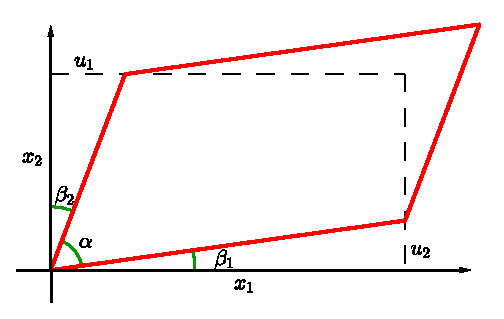
\includegraphics[scale=1.4]{deforma_formato}
\caption{\textit{Exemplo em duas dimens\~oes de como algumas componentes do tensor de deforma\c{c}\~ao promove a varia\c{c}\~ao no formato do meio.}}
\label{fig.deforma_formato}
\end{figure}
O angulo reto inicialmente formado pelos eixos coordenados $x_1$ e $x_2$ \'e reduzido a um \^angulo $\alpha$ que obedece \`a rela\c{c}\~ao
\begin{equation*}
\alpha=\frac{\pi}{2}-\beta_1-\beta_2,
\end{equation*}
onde $\beta_1$ e $\beta_2$ s\~ao os \^angulos formados pelos lados do paralelogramo e os eixos $x_1$ e $x_2$, respectivamente. Como a varia\c{c}\~ao angular \'e bastante pequena, temos que cada \^angulo $\beta_i$ pode ser aproximado por sua respectiva tangente, e considerando deslocamentos infinitesimais, temos
\begin{align*}
\beta_1+\beta_2&\approx\tan(\beta_1)+\tan(\beta_2)\\
&=\frac{\partial u_2}{\partial x_1}+\frac{\partial u_1}{\partial x_2}\\
&=2\epsilon_{12}=2\epsilon_{21}.
\end{align*}
Portanto, temos que o tensor de deforma\c{c}\~ao tamb\'em \'e respons\'avel pela altera\c{c}\~ao na dire\c{c}\~ao dos seguimentos que comp\~oem um corpo, mudando assim seu formato.


\subsection{Conserva\c{c}\~ao da Massa, Tens\~ao e o Equil\'ibrio do Momento Linear}\label{sec.massa_tensao_momen_lin}

O princ\'ipio de conserva\c{c}\~ao da massa \'e fundamental em mec\^anica do cont\'inuo na determina\c{c}\~ao da rela\c{c}\~ao entre o vetor de deslocamento $\mathbf{u}$ e a densidade de massa de um corpo $\rho$. Por defini\c{c}\~ao, a quantidade de massa ocupando um volume $V$  num dado tempo $t$ \'e
\begin{equation*}
m=\iiint_V\rho\,dV,
\end{equation*}
onde tanto a massa como a densidade n\~ao dependem apenas do tempo mas tamb\'em da posi\c{c}\~ao $\mathbf{x}$. Fixado um volume $V$, a taxa de varia\c{c}\~ao da massa no tempo \'e dada por
\begin{equation}\label{eq.massa_1}
\frac{d}{dt}m=\iiint_V\frac{\partial\rho}{\partial t}dV.
\end{equation}
Assumindo que n\~ao h\'a destrui\c{c}\~ao nem produ\c{c}\~ao de massa dentro do volume, a varia\c{c}\~ao da massa se d\'a apenas pelo quantidade de massa que passa pelo volume, ou que passa atrav\'es de uma das superf\'icies que limita esse volume, o que pode ser escrito como
\begin{equation}\label{eq.massa_2}
\frac{dm}{dt}=-\iint_S\rho\,\mathbf{v}\cdot d\mathbf{S},
\end{equation}
onde $\mathbf{v}$ \'e a velocidade da quantidade de massa que atravessa a superf\'icie $S$. A superf\'icie infinitesimal $dS$ \'e pequena o suficiente para ser considerada plana e tem o mesmo fluxo de massa em todos os seus pontos, e o sinal negativo decorre do fato de que o vetor normal \`a superf\'icie aponta no sentido de sa\'ida do volume. 

Substituindo a equa\c{c}\~ao \ref{eq.massa_2} na equa\c{c}\~ao \ref{eq.massa_1} temos
\begin{equation}\label{eq.massa_3}
\iiint_V\frac{\partial\rho}{\partial t}dV=-\iint_S\rho\,\mathbf{v}\cdot d\mathbf{S},
\end{equation}
ou seja, a taxa de varia\c{c}\~ao da quantidade de massa num determinado volume \'e proporcional \`a taxa de varia\c{c}\~ao da quantidade de massa que atravessa a superf\'icie que limita esse volume. Pelo teorema do divergente temos que
\begin{equation}\label{eq.massa_divergente}
\iint_S\rho\,\mathbf{v}\cdot d\mathbf{S}=\iiint_V\nabla\cdot (\rho\,\mathbf{v})\,dV,
\end{equation}
onde substiutindo a equa\c{c}\~ao \ref{eq.massa_divergente} na equa\c{c}\~ao \ref{eq.massa_3} e agrupando os integrandos sob um mesmo volume, temos
\begin{equation*}
\iiint_V\left[\frac{\partial\rho}{\partial t}+\nabla\cdot (\rho\,\mathbf{v})\right]\,dV=0,
\end{equation*}
que \'e a equa\c{c}\~ao que descreve a \textit{conserva\c{c}\~ao de massa} num determinado volume $V$.

Em geral, as for\c{c}as agindo no interior de um meio continuo s\~ao as chamadas \textit{for\c{c}as de superf\'icie}, ou seja, quando um material \'e submetido ao contato de uma carga em sua superf\'ice, for\c{c}as internas se propagam no inteiror do material atrav\'es de outras superf\'icies imagin\'arias provocando a deforma\c{c}\~ao desse material. Assim, podemos definir a \textit{tens\~ao} como o conjunto dessas for\c{c}as de superf\'ice, fazendo com que tens\~ao e deforma\c{c}\~ao estejam diretamente relacionadas. Matematicamente, tens\~ao media \'e definida como a for\c{c}a por unidade de \'area
\begin{equation}\label{eq.tensao_media}
\mathbf{\overline{T}}=\frac{\Delta\mathbf{F}}{\Delta S},
\end{equation}
e segundo o princ\'ipio fundamental da mec\^anica do cont\'inuo estabelecido por Cauchy, existe o limite para o valor da tens\~ao quando $\Delta S\to 0$,
\begin{equation*}
\mathbf{T}^{\mathbf{n}}=\lim_{\Delta S\to 0}\frac{\Delta\mathbf{F}}{\Delta S}=\frac{d\mathbf{F}}{dS}.
\end{equation*}
O vetor $\mathbf{n}$ \'e normal a superf\'icie de aplica\c{c}\~ao da tens\~ao $\mathbf{T}^{\mathbf{n}}$ e \'e \'util para identificar que determinada tens\~ao se aplica a determinada superf\'icie.

Al\'em das for\c{c}as de superf\'icie temos tamb\'em as for\c{c}as de corpo que agem \`a dist\^ancia como a for\c{c}a gravitacional ou a for\c{c}a el\'etrica que agem sobre um corpo material ou sobre uma carga el\'etrica, respectivamente. Denotando tal for\c{c}a por $\mathbf{f}(\mathbf{x},t)$ temos que a for\c{c}a total atuando num corpo \'e
\begin{equation}\label{eq.forca_total}
\mathbf{F}_T=\iint_S\mathbf{T}\,dS+\iiint_V\mathbf{f}\,dV,
\end{equation}
onde $V$ \'e o volume enclausurado pela superf\'icie $S$. Usando a defini\c{c}\~ao de for\c{c}a dada pela segunda lei de Newton, podemos reescrever a equa\c{c}\~ao \ref{eq.forca_total} como
\begin{equation}\label{eq.forca_total_2}
\frac{d}{dt}\iiint_V\rho\frac{d\mathbf{u}}{dt}\,dV=\iint_S\mathbf{T}\,dS+\iiint_V\mathbf{f}\,dV,
\end{equation}
onde $\mathbf{u}$ \'e o vetor deslocamento. A equa\c{c}\~ao \ref{eq.forca_total_2} estabelece o equil\'ibrio do \textit{momento linear}, ou seja, a taxa de varia\c{c}\~ao do momento linear de uma part\'icula no meio cont\'inuo \'e igual ao somat\'orio de for\c{c}as externas agindo nessa part\'icula. Discretizando a \'ultima integral da equa\c{c}\~ao acima podemos escrever
\begin{equation*}
\frac{1}{2}\sum_{i=1}^n\sum_{j=1}^n(\mathbf{F}_{ji}+\mathbf{F}_{ij}),
\end{equation*}
onde $\mathbf{F}_{ji}$ \'e a for\c{c}a exercida na part\'icula $i$ devida \`a part\'icula $j$. Pela terceira lei de Newton, for\c{c}as entre part\'iculas tem mesma intensidade e dire\c{c}\~ao e sentidos opostos, assim, $\mathbf{F}_{ji}=-\mathbf{F}_{ij}$. Mais ainda, uma part\'icula n\~ao exerce uma for\c{c}a em si mesma, ent\~ao $\mathbf{F}_{ii}=0$. Portanto, a equa\c{c}\~ao \ref{eq.forca_total_2} se resume a
\begin{equation*}
\frac{d}{dt}\iiint_V\rho\frac{d\mathbf{u}}{dt}\,dV=\iint_S\mathbf{T}\,dS.
\end{equation*}
Somente for\c{c}as externas s\~ao respons\'aveis por altera\c{c}\~oes no momento linear.

\subsection{O Tensor de Tens\~oes}\label{sec.tensor_tensoes}

Para deriva\c{c}\~ao do tensor de tens\~oes vamos utilizar o argumento do tetraedro de Cauchy, estudando as for\c{c}as agindo no inteiror de um meio cont\'inuo em rela\c{c}\~ao a um plano imagin\'ario com orienta\c{c}\~ao arbitr\'aria. O tetraedro \'e limitado pelos $O(0,0,0)$, $X(x,0,0)$, $Y(0,y,0)$ e $Z(0,0,z)$, contendo faces ortogonais, $OYZ$, $XOZ$ e $XYO$ e a face obl\'iqua $XYZ$, conforme a figura \ref{fig.tetraedro}.
\begin{figure}
\centering
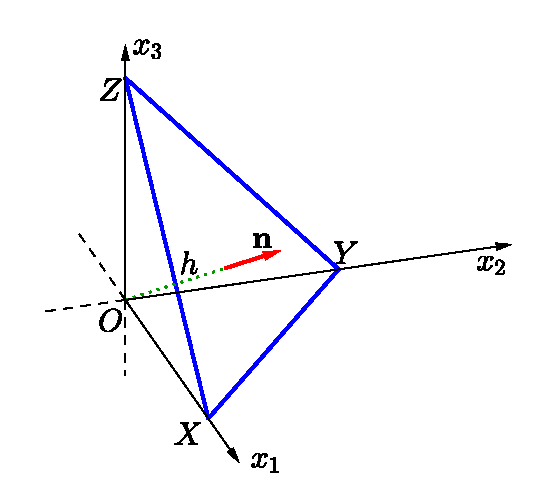
\includegraphics[scale=1]{tetraedro_cauchy}
\caption{\textit{Tetraedro de Cauchy, com for\c{c}as superficiais agindo em cada uma das faces ortogonais e na face obl\'iqua.}}
\label{fig.tetraedro}
\end{figure}

 Utilizando o equil\'ibro do momento linear dado pela equa\c{c}\~ao \ref{eq.forca_total_2}, podemos determinar a for\c{c}a agindo na face obl\'iqua de \'area $\Delta S$, considerando um tetraedro de dimens\~oes finitas.
\begin{equation}\label{eq.forca_total_3}
\overline{\rho}\,\Delta V\frac{d\overline{\mathbf{v}}}{dt}=\Delta \mathbf{F}+\Delta\mathbf{F}^{(\mathbf{e}_1)}+\Delta\mathbf{F}^{(\mathbf{e}_2)}+\Delta\mathbf{F}^{(\mathbf{e}_3)}+\overline{f}\Delta V,
\end{equation} 
onde $\Delta\mathbf{F}$ \'e a for\c{c}a superficial agindo na face obl\'iqua, $\Delta\mathbf{F}^{(\mathbf{e}_i)}$ \'e a for\c{c}a superficial agindo na face ortogonal cujo a normal \'e o eixo $x_i$, $\overline{f}$ \'e a for\c{c}a de campo agindo no tetraedro de volume $\Delta V$ e densidade $\rho$, e $\frac{d\overline{\mathbf{v}}}{dt}$ \'e a velocidade usada no c\'alculo da taxa de varia\c{c}\~ao do momento linear. As barras acima de cada s\'imbolo significam valores m\'edios para tetraedros de dimens\~oes finitas. Substituindo a equa\c{c}\~ao \ref{eq.tensao_media} na equa\c{c}\~ao \ref{eq.forca_total_3} temos
\begin{equation}\label{eq.forca_total_4}
\overline{\rho}\,\Delta V\frac{d\overline{\mathbf{v}}}{dt}=\mathbf{\overline{T}}^{(\mathbf{n})}\,\Delta S-\mathbf{\overline{T}}^{(\mathbf{e}_1)}\,\Delta S_1-\mathbf{\overline{T}}^{(\mathbf{e}_2)}\,\Delta S_2-\mathbf{\overline{T}}^{(\mathbf{e}_3)}\,\Delta S_3+\overline{f}\,\Delta V,
\end{equation}
onde $\Delta S_i$ \'e a \'area da face cujo a normal \'e o eixo $x_i$. Note, ainda pela figura \ref{fig.tetraedro}, que as faces ortogonais tem suas respectivas normais com a mesma dire\c{c}\~ao mas sentido oposto ao respectivo vetor unit\'ario $\mathbf{e}_i$ do eixo correspondente, da\'i o sinal negativo na equa\c{c}\~ao acima por conta da terceira lei de Newton. Para continuarmos nossa deriva\c{c}\~ao precisamos relacionar a \'area da face obl\'iqua com as \'areas das faces ortogonais. Observe que cada componente $n_i$ do vetor $\mathbf{n}$ \'e, por defini\c{c}\~ao,
\begin{align*}
n_1&=\mathbf{n}\cdot\mathbf{e}_1=\norm{\mathbf{n}}\,\norm{\mathbf{e}_1}\cos(X\hat{O}N)\\
n_2&=\mathbf{n}\cdot\mathbf{e}_2=\norm{\mathbf{n}}\,\norm{\mathbf{e}_2}\cos(Y\hat{O}N)\\
n_3&=\mathbf{n}\cdot\mathbf{e}_3=\norm{\mathbf{n}}\,\norm{\mathbf{e}_3}\cos(Z\hat{O}N)\\
\end{align*}
Usando a defini\c{c}\~ao de cosseno nos tri\^angulos $XON$, $YON$ e $ZON$ temos que
\begin{equation*}
h=\overline{XO}\,n_1=\overline{YO}\,n_2=\overline{ZO}\,n_3,
\end{equation*}
e calculando o volume do tetraedro em rela\c{c}\~ao a cada uma das faces temos
\begin{equation}\label{eq.volume_tetraedro}
\Delta V=\frac{1}{3}h\,\Delta S=\frac{1}{3}\overline{XO}\Delta S_1=\frac{1}{3}\overline{YO}\Delta S_2=\frac{1}{3}\overline{ZO}\Delta S_3,
\end{equation}
e da\'i temos a rela\c{c}\~ao entre as \'areas,
\begin{equation}\label{eq.relacao_areas}
\Delta S=\Delta S_in_i,\quad\text{onde}\quad i=1,2,3.
\end{equation}
Usando as equa\c{c}\~oes \ref{eq.volume_tetraedro} e \ref{eq.relacao_areas} podemos escrever a equa\c{c}\~ao \ref{eq.forca_total_4} como
\begin{equation*}
\overline{\rho}\,\frac{1}{3}h\,\Delta S\frac{d\overline{\mathbf{v}}}{dt}=\mathbf{\overline{T}}^{(\mathbf{n})}\,\Delta S-\mathbf{\overline{T}}^{(\mathbf{e}_1)}\,n_1\,\Delta S-\mathbf{\overline{T}}^{(\mathbf{e}_2)}\,n_2\,\Delta S-\mathbf{\overline{T}}^{(\mathbf{e}_3)}\,n_3\,\Delta S+\overline{f}\,\frac{1}{3}h\,\Delta S.
\end{equation*}
Cancelando $\Delta S$, temos
\begin{equation*}
\overline{\rho}\,\frac{1}{3}h\frac{d\overline{\mathbf{v}}}{dt}=\mathbf{\overline{T}}^{(\mathbf{n})}-\mathbf{\overline{T}}^{(\mathbf{e}_1)}\,n_1-\mathbf{\overline{T}}^{(\mathbf{e}_2)}\,n_2-\mathbf{\overline{T}}^{(\mathbf{e}_3)}\,n_3+\overline{f}\frac{1}{3}h.
\end{equation*}
Reduzindo o tetraedro de dimens\~oes finitas a um tetraedro infinitesimal, fazemos $h\to 0$ mantendo o v\'ertice $O$ centrado na origem e sem alterar a dire\c{c}\~ao de $h$,
\begin{equation*}
\mathbf{T}^{(\mathbf{n})}=\mathbf{T}^{(\mathbf{e}_1)}\,n_1+\mathbf{T}^{(\mathbf{e}_2)}\,n_2+\mathbf{T}^{(\mathbf{e}_3)}\,n_3.
\end{equation*}
Em termos matriciais, temos
\begin{align}\nonumber
\mathbf{T}^{(\mathbf{n})}&=
\begin{bmatrix}
T_1^{(\mathbf{e}_1)}\\
T_2^{(\mathbf{e}_1)}\\
T_3^{(\mathbf{e}_1)}
\end{bmatrix}
n_1+
\begin{bmatrix}
T_1^{(\mathbf{e}_2)}\\
T_2^{(\mathbf{e}_2)}\\
T_3^{(\mathbf{e}_2)}
\end{bmatrix}
n_2+
\begin{bmatrix}
T_1^{(\mathbf{e}_3)}\\
T_2^{(\mathbf{e}_3)}\\
T_3^{(\mathbf{e}_3)}
\end{bmatrix}
n_3\\\label{eq.matriz_tensao}
&=
\begin{bmatrix}
T_1^{(\mathbf{e}_1)}&T_1^{(\mathbf{e}_2)}&T_1^{(\mathbf{e}_3)}\\
T_2^{(\mathbf{e}_1)}&T_2^{(\mathbf{e}_2)}&T_2^{(\mathbf{e}_3)}\\
T_3^{(\mathbf{e}_1)}&T_3^{(\mathbf{e}_2)}&T_3^{(\mathbf{e}_3)}
\end{bmatrix}
\begin{bmatrix}
n_1\\
n_2\\
n_3
\end{bmatrix}.
\end{align}
Ou seja, se sabemos as tens\~oes em tr\^es planos mutuamente ortogonais com rela\c{c}\~ao a um determinado ponto $P$, podemos determinar a tens\~ao num outro plano qualquer passando por $P$.

Definindo a matrix
\begin{equation*}
\tau=
\begin{bmatrix}
\tau_{11}&\tau_{12}&\tau_{13}\\
\tau_{21}&\tau_{22}&\tau_{23}\\
\tau_{31}&\tau_{32}&\tau_{33}
\end{bmatrix},
\end{equation*}
onde cada componente $\tau_{ij}$ representa a j-\'esima componente da for\c{c}a superficial agindo no plano cuja normal tem mesma dire\c{c}\~ao do eixo $x_i$. Assim, comparando a matriz da equa\c{c}\~ao \ref{eq.matriz_tensao} com a matriz $\tau$ e considerando as defini\c{c}\~oes dadas para os \'indices, vemos que
\begin{equation*}
\tau_{ij}=T_j^{(\mathbf{e}_i)},
\end{equation*}
ou seja, a equa\c{c}\~ao \ref{eq.matriz_tensao} pode ser escrita compactamente como
\begin{equation}\label{eq.tensor_tau}
\mathbf{T}^{(\mathbf{n})}=\tau^\top\mathbf{n}.
\end{equation}
A matriz $\tau$ \'e chamada de \textit{tensor de tens\~oes de Cauchy}, o s\'imbolo $\top$ indica transposi\c{c}\~ao e $\mathbf{T}^{(\mathbf{n})}$ \'e a tens\~ao aplicada em um plano qualquer com orienta\c{c}\~ao $\mathbf{n}$. Utilizando a nota\c{c}\~ao de somat\'orio podemos escrever a equa\c{c}\~ao \ref{eq.tensor_tau} na forma
\begin{equation}\label{eq.somatorio_tensor_tau}
\mathbf{T}^{(\mathbf{n})}=\sum_{j=1}^3\tau_{ji}n_j,\quad \text{para}\quad i=1,2,3.
\end{equation}

\subsection{Equa\c{c}\~ao do Movimento de um Corpo El\'astico e Cont\'inuo}

Para deduzir a equa\c{c}\~ao do movimento vamos fazer uso do conceito de equil\'ibrio do momento linear estabelecido na subse\c{c}\~ao \ref{sec.massa_tensao_momen_lin} e da defini\c{c}\~ao do tensor de tens\~oes estabelacido na subse\c{c}\~ao \ref{sec.tensor_tensoes}. Assim, substituindo a equa\c{c}\~ao \ref{eq.somatorio_tensor_tau} na equa\c{c}\~ao \ref{eq.forca_total_2} temos
\begin{align*}
\iiint_V\rho\frac{d^2\mathbf{u}}{dt^2}\,dV&=\iint_S\mathbf{T}\,dS+\iiint_V\mathbf{f}\,dV\\
\iiint_V\rho\frac{d^2u_i}{dt^2}\,dV&=\iint_S\sum_{j=1}^3\tau_{ji}n_jdS+\iiint_Vf_i\,dV,\quad \text{para}\quad i=1,2,3.
\end{align*}
Para escrever todas as integrais como integral de volume vamos usar o teorema do divergente,
\begin{equation}
\iiint_V\rho\frac{d^2u_i}{dt^2}\,dV=\iiint_V\sum_{j=1}^3\frac{\partial\tau_{ji}}{\partial x_j}dV+\iiint_Vf_i\,dV,\quad \text{para}\quad i=1,2,3
\end{equation}
e como os volumes s\~ao os mesmos em cada integral, podemos usar a linearidade da integra\c{c}\~ao e escrever
\begin{equation}
\iiint_V\left(\sum_{j=1}^3\frac{\partial\tau_{ji}}{\partial x_j}dV+f_i-\rho\frac{d^2u_i}{dt^2}\right)dV=0,\quad \text{para}\quad i=1,2,3.
\end{equation}
Para satisfazer essa integral o integrando deve ser nulo, de onde podemos concluir que
\begin{equation}
\sum_{j=1}^3\frac{\partial\tau_{ji}}{\partial x_j}dV+f_i=\rho\frac{d^2u_i}{dt^2},\quad \text{para}\quad i=1,2,3.
\end{equation}
Essa equa\c{c}\~ao \'e conhecida como a \textit{equa\c{c}\~ao do movimento de Cauchy} ou \textit{primeira lei do movimento de Cauchy}, e relaciona dois tipos de for\c{c}a, superficial e de corpo, com a acelera\c{c}\~ao de um corpo num meio cont\'inuo e el\'astico. Ou seja, a acelera\c{c}\~ao de um corpo num meio cont\'inuo e el\'astico resulta da aplica\c{c}\~ao desses dois tipos de for\c{c}a.

  
\section{Equações de Lamé}
\subsection{Rela\c{c}\~oes Constitutivas}

As rela\c{c}\~oes contitutivas, ou rela\c{c}\~oes de tens\~ao-deforma\c{c}\~ao, foram estabelecidas experimentalmente e descrevem como as for\c{c}as aplicadas em materiais el\'asticos est\~ao linearmente relacionadas com a deforma\c{c}\~ao observada nesses materiais. As rela\c{c}\~oes consitutivas s\~ao conhecidas tamb\'em como a lei de Hooke, a qual estabelece que cada componente do tensor de tens\~oes est\'a linearmente relacionada com todas as componentes do tensor de deforma\c{c}\~oes. Dessa forma, a lei de Hooke pode ser escrita como
\begin{equation}\label{eq.lei_hooke}
\sigma_{ij}=\sum_{k=1}^3\sum_{l=1}^3c_{ijkl}\,\varepsilon_{kl}
\end{equation}
onde $i,j = 1,2,3$ e $c$ \'e constante.
Dadas as simetrias de ambos os tensores, a lei de Hooke pode ser escrita na forma matricial contendo seis equa\c{c}\~oes independentes. Para isso, vamos realizar uma mudan\c{c}a de \'indices criando uma lista ordenada com os pares ordenados $(i,j)$ onde $i\le j$, e considerando o n\'umero $m = 1,2,3,4,5,6$ que d\'a a posi\c{c}\~ao de cada par nessa lista. Assim, temos que os poss\'iveis pares ordenados s\~ao substituidos pelos seguintes valores de $m$
\begin{equation*}
(1,1)\rightarrow 1\quad (2,2)\rightarrow 2\quad (3,3)\rightarrow 3\quad (2,3)\rightarrow 4\quad (1,3)\rightarrow 5\quad (1,2)\rightarrow 6. 
\end{equation*}
Ou seja, estamos fazendo a substitui\c{c}\~ao $(i,j)\rightarrow m$ com 
\begin{empheq}[left=\empheqlbrace]{align*}
m&=i&\text{se}\quad i=j\\
m&=9-(i+j)&\text{se}\quad i\neq j.
\end{empheq}
Analogamente, podemos fazer a substitui\c{c}\~ao dos \'indices $(k,l)\rightarrow n$ e escrever $c_{ijkl}$ como $C_{mn}$, obtendo a \textit{matriz de elasticidade} $C=C_{mn}$ com $m,n \in \left\{1,2,3,4,5,6\right\}$.
Dessa forma, as equa\c{c}\~oes de tens\~ao-deforma\c{c}\~ao definidas em \ref{eq.lei_hooke} podem ser escritas na forma matricial como
\begin{equation*}
\begin{bmatrix}
\sigma_{11}\\
\sigma_{22}\\
\sigma_{33}\\
\sigma_{23}\\
\sigma_{13}\\
\sigma_{12}
\end{bmatrix}=
\begin{bmatrix}
C_{11}&C_{12}&C_{13}&C_{14}&C_{15}&C_{16}\\
C_{21}&C_{22}&C_{23}&C_{24}&C_{25}&C_{26}\\
C_{31}&C_{32}&C_{33}&C_{34}&C_{35}&C_{36}\\
C_{41}&C_{42}&C_{43}&C_{44}&C_{45}&C_{46}\\
C_{51}&C_{52}&C_{53}&C_{54}&C_{55}&C_{56}\\
C_{61}&C_{62}&C_{63}&C_{64}&C_{65}&C_{66}
\end{bmatrix}
\begin{bmatrix}
\varepsilon_{11}\\
\varepsilon_{22}\\
\varepsilon_{33}\\
2\,\varepsilon_{23}\\
2\,\varepsilon_{13}\\
2\,\varepsilon_{12}
\end{bmatrix}.
\end{equation*}
Podemos notar que, por conta da simetria dos tensores de tens\~ao e de deforma\c{c}\~ao, basta considerar apenas seis das nove equa\c{c}\~oes iniciais dadas pela rela\c{c}\~ao \ref{eq.lei_hooke}.

\subsection{Os Par\^ametros de Lam\'e}

Considere um material com determinadas caracter\'isticas e com posi\c{c}\~ao medida em rela\c{c}\~ao a um determinado sistema de coordenadas. Podemos alterar o sistema de coordenadas sem alterar as caracter\'isticas do material em quest\~ao. Essa invari\^ancia das caracter\'isticas de um corpo em rela\c{c}\~ao a uma mudan\c{c}a no sistema de coordenadas \'e chamada \textit{simetria material}. Num certo sistema de coordenadas, a matriz de elasticidade nos permite reconhecer qual o tipo de simetria que um corpo apresenta (s\~ao oito no total), pois uma altera\c{c}\~ao no sistema de coordenadas gera um efeito nas equa\c{c}\~oes de tens\~ao-deforma\c{c}\~ao.  Ainda mais, sob determinadas condi\c{c}\~oes, a matriz de elasticidade \'e invariante para algumas altera\c{c}\~oes no sistema de coordenadas.
Estamos interessados em transforma\c{c}\~ao de coordenadas que preservam dist\^ancias entre pontos, ou seja as rota\c{c}\~oes e reflex\~oes, tamb\'em conhecidas como \textit{tansforma\c{c}\~oes ortogonais}. Dado um ponto $\mathbf{x}\in\mathbb{R}^3$, uma transforma\c{c}\~ao ortogonal \'e dada por uma matriz $A_{3\times 3}$ onde 
\begin{equation*}
\mathbf{\hat{x}}=A\,\mathbf{x},
\end{equation*} 
com $A^\top A=I$, ou $A^\top=A^{-1}$, e $I$ \'e a matriz identidade $3\times 3$.
O conjunto de todas as transforma\c{c}\~oes ortogonais $A$ que n\~ao alteram as caracter\'isticas el\'asticas de um meio cont\'inuo s\~ao chamadas \textit{grupo de simetria}. Dentre os grupos de simetria, o que nos interessa \'e o caso \textit{isotr\'opico cont\'inuo}, que cont\'em todas as transforma\c{c}\~oes ortogonais usadas nas deriva\c{c}\~oes dos grupos anteriores, fazendo com que qualquer sistema de coordenadas seja efetivo no estudo das caracter\'isticas el\'asticas de um meio n\~ao sendo necess\'aria uma orienta\c{c}\~ao em particular. Assim, atrav\'es dos grupos de simetria anteriores, podemos demonstrar que a matriz de elasticidade para o grupo isotr\'opico cont\'inuo \'e
\begin{equation}
C_{iso}=
\begin{bmatrix}
\lambda +2\,\mu & \lambda & \lambda &0&0&0\\
\lambda&\lambda+2\,\mu&\lambda&0&0&0\\
\lambda&\lambda&\lambda+2\,\mu&0&0&0\\
0&0&0&\mu&0&0\\
0&0&0&0&\mu&0\\
0&0&0&0&0&\mu
\end{bmatrix},
\end{equation} 
onde os par\^ametros $\lambda$ e $\mu$ s\~ao conhecidos como os \textit{par\^ametros de Lam\'e}, e est\~ao estreitamente relacionados aos autovalores da matriz $C_{iso}$. Fisicamente, $\mu$ est\'a relacionado com a rigidez do s\'olido em quest\~ao e $\lambda$ com sua compressibilidade.

\subsection{Condi\c{c}\~oes de Contorno}

Vimos que a matriz de elasticidade para meios isotr\'opicos possui os par\^ametros $\lambda$ e $\mu$ que definem as caracter\'isticas el\'asticas do meio. Uma mudan\c{c}a abrupta nesses par\^ametros indica uma altera\c{c}\~ao na composi\c{c}\~ao do meio de propaga\c{c}\~ao da deforma\c{c}\~ao, indicando que a mesma atravessou uma superf\'icie de contato entre duas camadas de subsuperf\'icie. Vamos analisar como a descontinuidade dos par\^ametros de Lam\'e afetam os tensores de tens\~ao e de deforma\c{c}\~ao.
 
Dados dois meios $M_1$ e $M_2$ com caracter\'isticas el\'asticas distintas contidos no espa\c{c}o $\mathbb{R}^3$, separados por uma superf\'icie de contato $S$ com dire\c{c}\~ao normal $\mathbf{n}$. Sendo $\mathbf{F}$ o campo de for\c{c}as de contato, $\mathbf{p}_0\in S$, $\mathbf{p}_1\in M_1$ e $\mathbf{p}_2\in M_2$, queremos calcular a diferen\c{c}a entre os limites de $\mathbf{F}$ aplicada a $\mathbf{p}_1$ e $\mathbf{p}_2$ quando esses pontos tendem a $\mathbf{p}_0$ atrav\'es dos meios $M_1$ e $M_2$, respectivamente. Ou seja, queremos calcular o salto de $\mathbf{F}$ em $\mathbf{p}_0$ e assumindo que os limites parciais existem, temos
\begin{equation*}
\left[\left[\mathbf{F}\right]\right]=\lim_{\mathbf{p}_1\to\mathbf{p}_0}\mathbf{F}(\mathbf{p}_1)-\lim_{\mathbf{p}_2\to\mathbf{p}_0}\mathbf{F}(\mathbf{p}_2).
\end{equation*}
Fixado um ponto $\mathbf{p}_0\in S$ qualquer vamos utilizar um cilindro infinitesimal centrado em $\mathbf{p}_0$, com altura $dh$ e \'area das bases $dA$, com orienta\c{c}\~ao normal $\mathbf{n}$ e onde cada metade do cilindro se encontra nos meios $M_1$ e $M_2$ conforme a figura \ref{fig.interface_elastici}. 
\begin{figure}[!htb]
\centering
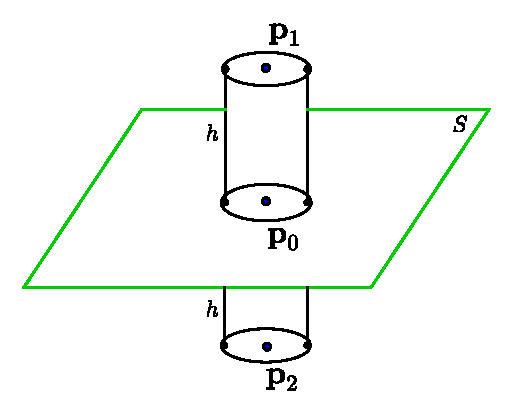
\includegraphics[scale=1]{interface_elastici}
\caption{\textit{Cilindro de dimens\~oes infinitesimais dividido pela interface separadora dos meios 1 e 2.}}
\label{fig.interface_elastici}
\end{figure}
Considerando ainda que cada um dos pontos $\mathbf{p}_1$ e $\mathbf{p}_2$ s\~ao os centros de cada uma das bases do cilindro, temos que os pontos $\mathbf{p}_0$, $\mathbf{p}_1$ e $\mathbf{p}_2$ est\~ao alinhados. Utilizando novamente a equa\c{c}\~ao \ref{eq.forca_total_3} e desprezando as for\c{c}as aplicadas na parede do cilindro (j\'a que vamos fazer $h\to 0$), temos que o equil\'ibrio de for\c{c}as aplicadas ao cilindro \'e dado por 
\begin{equation*}
\mathbf{F}=\mathbf{F}(\mathbf{p}_1)+\mathbf{F}(\mathbf{p}_2)+f
\end{equation*} 
onde $f$ \'e uma for\c{c}a de campo. Utilizando a segunda lei de Newton, utilizando a equa\c{c}\~ao \ref{eq.tensao_media} e desprezando as for\c{c}as de campo, temos
\begin{equation*}
\rho\,dh\,dA\frac{d\mathbf{v}}{dt}=\mathbf{T}(\mathbf{p}_1,\mathbf{n})dA+\mathbf{T}(\mathbf{p}_2,-\mathbf{n})dA.
\end{equation*} 
Fazendo o limite quando $h\to 0$ e mantendo constantes as \'areas das bases do cilindro, temos que os pontos $\mathbf{p}_i$ convergem para $\mathbf{p}_0$, e a equa\c{c}\~ao acima se torna
\begin{equation*}
\mathbf{T}(\mathbf{p}_0,\mathbf{n})-\mathbf{T}(\mathbf{p}_0,\mathbf{n})=\mathbf{0}.
\end{equation*}
Como o ponto $\mathbf{p}_0$ \'e tomado arbitrariamente, temos que o salto do tensor de tens\~oes ao longo da superf\'icie $S$ \'e nulo
\begin{equation*}
\left[\left[\mathbf{T}\right]\right]=\mathbf{0}.
\end{equation*}
Considerando um modelo onde uma camada n\~ao vai invadir a outra temos que a componente normal do vetor de deslocamento $\mathbf{u}\in S$ \'e nula. Da mesma forma, considerando que uma camada n\~ao desliza sobre a outra, temos que as componentes tangenciais de $\mathbf{u}$ tamb\'em s\~ao zero, e da\'i assumimos que o salto de $\mathbf{u}$ \'e nulo bem como sua velocidade,
\begin{equation*}
\left[\left[\mathbf{u}\right]\right]=\mathbf{0}\quad\text{e}\quad\left[\left[\frac{\partial}{\partial t}\mathbf{u}\right]\right]=\mathbf{0}.
\end{equation*}



\section{Generalizações da teoria}

\section{Conclusões}
\chapter{Acoplamento Magneto-e\'alstico}

\section{Introdu\c{c}\~ao}

Como vimos na subse\c{c}\~ao \ref{sec.fund_eletr}, quando uma estrutura condutiva se movimenta num campo magn\'etico, uma corrente el\'etrica e um campo magn\'etico vari\'avel s\~ao gerados nessa estrutura. Segundo \cite{Mikhailenko_1997}, a passagem de uma onda s\'ismica pela subsuperf\'icie terrestre gera o movimento do material que comp\~oe essa subsuperf\'icie. Considerando que esse material \'e cont\'inuo e el\'astico, cont\'em uma certa distribui\c{c}\~ao de cargas el\'etricas e que o planeta Terra possui um campo geomagn\'etico natural, temos que o movimento relativo entre o material e o campo geomagn\'etico vai gerar varia\c{c}\~oes geomagn\'eticas locais associadas \`as ondas s\'ismicas que provocaram o movimento do material. Mais ainda, segundo \cite{Anisimov_1985} e \cite{Sadovsky_1980}, a onda eletromagn\'etica induzida \'e ''congelada`` \`a onda s\'ismica e se propaga n\~ao com a velocidade da luz, mas com a velocidade da onda $P$ ou da onda $S$, dependendo do tipo de onda s\'ismica, e podemos registrar e estudar essa varia\c{c}\~ao geomagn\'etica.
Um corpo nessas condi\c{c}\~oes \'e chamado de s\'olidos eletromagn\'etico-el\'asticos, essas varia\c{c}\~oes no campo geomagn\'etico s\~ao chamadas de \textit{ondas sismomagn\'eticas} e esse efeito recebeu o nome de \textit{efeito sismomagn\'etico} ou \textit{efeito magnetoel\'astico}.

Segundo \cite{erigen_1963}, \'e poss\'ivel investigar algumas intera\c{c}\~oes din\^amicas que podem ocorrer entre campos eletromagn\'eticos e campos el\'asticos em s\'olidos homog\^eneos e isotr\'opicos. Assim, esses autores desenvolveram um modelo matem\'atico de combina\c{c}\~ao entre a teoria de elasticidade infinitesimal e a teoria eletromagn\'etica linearizada, o qual ser\'a apresentado a seguir. A intera\c{c}\~ao se deve principalmente \`a for\c{c}a de corpo de Lorentz, \`a modifica\c{c}\~ao das equa\c{c}\~oes constitutivas e das condi\c{c}\~oes de contorno provocada pela velocidade do material, e \`as for\c{c}as superficiais introduzidas pelos campos.

\section{Equa\c{c}\~oes Constitutivas do Meio}
Seguindo a nota\c{c}\~ao apresentada em \cite{erigen_1963}, temos que os vetores eletromagn\'eticos que representam o meio de propaga\c{c}\~ao das ondas propriamnte dito s\~ao representados por $\mathbf{E}^0$, $\mathbf{D}^0$, $\mathbf{B}^0$, $\mathbf{H}^0$ e
$\mathbf{J}^0$. Essas mesmas quantidades, quando se referirem \`as medidas observadas em laborat\'orio s\~ao denotadas apenas retirando-se o sobre-escrito $0$. Transferindo essa nota\c{c}\~ao para as equa\c{c}\~oes \ref{eq.D_funcao_E} e \ref{eq.B_funcao_H} temos
\begin{equation}\label{eq.constitutivas_parciais}
\mathbf{D}^0=\epsilon\,\mathbf{E}^0\quad\text{e}\quad\mathbf{B}^0=\mu\,\mathbf{H}^0.
\end{equation}

Em muitos materiais, a densidade de corrente el\'etrica \'e linearmente dependente de um campo el\'etrico externo, e tal rela\c{c}\~ao, conhecida como a \textit{lei de Ohm}, pode ser escrita usando a nota\c{c}\~ao apresentada acima como
\begin{equation}\label{eq.lei_ohm}
\mathbf{J}^0=\sigma\,\mathbf{E}^0,
\end{equation}
onde $\sigma$ \'e a \textit{condutividade} do meio. As equa\c{c}\~oes \ref{eq.constitutivas_parciais} juntamente com a equa\c{c}\~ao \ref{eq.lei_ohm} s\~ao denominadas \textit{equa\c{c}\~oes eletromagn\'eticas contitutivas do meio}, quando o mesmo \'e isotr\'opico, homog\^eneo e se encontra em repouso. As mesmas equa\c{c}\~oes se mant\^em quando o meio se move por ocasi\~ao da passagem de uma onda s\'ismica. 


\section{Modelo de Dunkin e Erigen}






\section{Conclusões}
\chapter{Recondicionamento do Modelo de Dunkin e Erigen}
Uma das contribui\c{c}\~oes dessa monografia \'e a utiliza\c{c}\~ao de hip\'oteses simplificadoras de ordem f\'isica e experimental, dispon\'iveis na literatura, para reeescrever o modelo do acoplamento magneto-el\'astico de forma que o mesmo possa receber um tratamento matem\'atico e computacional, no sentido de solucionar um problema direto.

Como vimos na subse\c{c}\~ao \ref{sec.magnetizacao_polarizacao}, a polariza\c{c}\~ao e magnetiza\c{c}\~ao de um determinado material depende das caracter\'isticas de cada material. De acordo com \cite{jackson_classical_1999} e \cite{griffiths}, as equa\c{c}\~oes constitutivas apresentadas na subse\c{c}\~ao \ref{sec.constitutivas_dunkin} podem n\~ao ser simples pois existe uma diversidade enorme de propriedades el\'etricas e magn\'eticas dos materias, especialmente em s\'olidos cristal\'inicos  e materias ferroel\'etricos e ferromagn\'eticos que t\^em polariza\c{c}\~ao e magnetiza\c{c}\~ao n\~ao nulos mesmo na absten\c{c}\~ao de aplica\c{c}\~ao de campos eletromagn\'eticos. Com excess\~ao desses tipos de materias, a aplica\c{c}\~ao de campos eletromagn\'eticos produzem polariza\c{c}\~ao e magnatiza\c{c}\~ao proporcional aos campos aplicados, e a rela\c{c}\~ao do campo de densidade de fluxo el\'etrico com o campo el\'etrico bem como a rela\c{c}\~ao do campo magn\'etico auxiliar com o campo magn\'etico s\~ao consideradas lineares, pois a contribui\c{c}\~ao das parcelas n\~ao-lineares tornam-se desprez\'iveis. Podemos ainda considerar a permeabilidade magn\'etica de muitos materiais tendo valor muito pr\'oximo da permeabilidade magn\'etica no v\'acuo, assim $\mu=\mu_0$. Com isso, temos que o escalar $\alpha$ definido em \ref{eq.constitutiva_1} tem seu valor considerado nulo, e as express\~oes para o campo de densidade de fluxo el\'etrico e o campo magn\'etico da subse\c{c}\~ao \ref{sec.constitutivas_dunkin} se tornam
\begin{align}\label{eq.constitutiva_alpha_1}
\mathbf{D}&=\epsilon\,\mathbf{E}\\\nonumber\\\label{eq.constitutiva_alpha_2}
\mathbf{B}&=\mu\,\mathbf{H}.
\end{align}
Substituindo a equa\c{c}\~ao \ref{eq.constitutiva_alpha_1} na equa\c{c}\~ao \ref{eq.campo_dunkin_1} e aplicando a transformada de Fourier, temos a rela\c{c}\~ao entre o campo el\'etrico e o campo magn\'etico auxiliar dada por
\begin{equation}
\nabla\times\mathbf{\widehat{E}}=i\,\omega\,\mu_0\mathbf{\widehat{H}},
\end{equation}
onde $i$ \'e um n\'umero complexo, $\omega$ \'e a frequ\^encia temporal e a nota\c{c}\~ao $\widehat{\,\,}$ significa que a fun\c{c}\~ao vetorial est\'a no dom\'inio da frequ\^encia temporal.

Ondas eletromagn\'eticas se propagam com velocidade da luz que \'e limitada. Segundo \cite{jackson_classical_1999}, num sistema onde as dimens\~oes s\~ao pequenas comparadas ao comprimento de onda eletromagn\'etica e comparadas \`a escala de tempo dominante, podemos tratar a velocidade da luz como instant\^anea num regime denominado \textit{quasi-estacion\'ario}. Como consequ\^encia dessa premissa, em meios condutivos a contribui\c{c}\~ao do campo de densidade de fluxo el\'etrico \'e muito pequena quando comparada \`a contribui\c{c}\~ao da densidade de corrente el\'etrica na produ\c{c}\~ao de campos magn\'eticos. Assim, podemos desprezar a parcela referente \`a corrente deslocada introduzida por Maxwell na lei de Amper\`e, o que implica (pela equa\c{c}\~ao \ref{eq.campo_dunkin_3}) em $\rho_e=0$. 
Vamos supor ainda que o campo magn\'etico auxiliar medido durante o efeito magneto-el\'astico seja uma combina\c{c}\~ao do campo magn\'etico gerado $\mathbf{H}$ mais o campo magn\'etico natural da Terra $\mathbf{H}^0$, e para manter a nota\c{c}\~ao vamos usar a substitui\c{c}\~ao 
\begin{equation}
\mathbf{H}\longrightarrow\mathbf{H}+\mathbf{H}^0.
\end{equation}
Utilizando a equa\c{c}\~ao \ref{eq.constitutiva_alpha_2}, o campo de densidade de corrente el\'etrica dado pela subse\c{c}\~ao \ref{sec.constitutivas_dunkin} poder ser reescrito como
\begin{equation}
\mathbf{J}=\sigma\,\mathbf{E}+\mathbf{v}\times\sigma\,\mu_0\mathbf{H}.
\end{equation}
Substituindo esta \'ultima rela\c{c}\~ao juntamente com a equa\c{c}\~ao \ref{eq.constitutiva_alpha_1} na equa\c{c}\~ao \ref{eq.campo_dunkin_2}, e aplicando a transformada de Fourier, temos
\begin{equation}
\nabla\times\mathbf{\widehat{H}}=(\sigma-i\,\epsilon\,\omega)\,\mathbf{\widehat{E}}+\mathbf{\widehat{v}}\times\sigma\mu_0\mathbf{H}^0,
\end{equation}
onde $\mathbf{\widehat{v}}=-i\,\omega\mathbf{\widehat{u}}$ \'e a velocidade de deslocamento do meio. Na dedu\c{c}\~ao da equa\c{c}\~ao acima, estamos considerando que a contribui\c{c}\~ao da parcela $\mathbf{\widehat{v}}\times\sigma\mu_0\mathbf{\widehat{H}}$ \'e desprez\'ivel se comparada \`a contribui\c{c}\~ao do campo geomagn\'etico, ainda como uma consequ\^encia do regime quasi-estacion\'ario.

De acordo com \cite{Knopoff_1955}, a altera\c{c}\~ao que o campos eletromagn\'eticos aplicam em ondas el\'asticas \'e desprez\'ivel, e assim podemos excluir a for\c{c}a de Lorentz e reescrever a equa\c{c}\~ao \ref{eq.campo_dunkin_5} no dom\'inio da frequ\^encia na forma matricial como 
\begin{equation}
-i\,\omega\rho\,\mathbf{\widehat{v}}=\nabla\cdot\widehat{\tau} + \mathbf{\widehat{F}}.
\end{equation}
A lei de Hooke dada na subse\c{c}\~ao \ref{sec.constitutivas_dunkin} pode ser reescrita no dom\'inio da frequ\^encia e em sua forma matricial como
\begin{equation}
\widehat{\tau}=\lambda\,\nabla\cdot\mathbf{\widehat{u}}\cdot\,I + \mu\,(\nabla\,\mathbf{\widehat{u}}+\nabla\mathbf{\widehat{u}}^\top),
\end{equation}
onde $I$ \'e a matriz identidade e $\nabla\mathbf{\widehat{u}}=(\nabla u_1,\nabla u_2,\nabla u_3)$ \'e o gradiente do campo vetorial que d\'a o deslocamento do meio de propaga\c{c}\~ao das ondas.

Substituindo a equa\c{c}\~ao \ref{eq.constitutiva_alpha_2} na equa\c{c}\~ao \ref{eq.campo_dunkin_4} e aplicando a transformada de Fourier, temos
\begin{equation}
\nabla\cdot\mathbf{\widehat{H}}=0.
\end{equation}

Assumindo as hip\'oteses simplificadoras acima, com a depend\^encia do tempo dada por $e^{(-i\,\omega\,t)}$, as equa\c{c}\~oes diferenciais parciais linearizadas de magneto-elasticidade s\~ao
\begin{align*}
\nabla\times\mathbf{\widehat{E}}&=i\,\omega\,\mu_0\mathbf{\widehat{H}}\\\\
\nabla\times\mathbf{\widehat{H}}&=(\sigma-i\,\epsilon\,\omega)\,\mathbf{\widehat{E}}+\mathbf{\widehat{v}}\times\sigma\mu_0\mathbf{H}^0\\\\
-i\,\omega\rho\,\mathbf{\widehat{v}}&=\nabla\cdot\widehat{\tau} + \mathbf{\widehat{F}}\\\\
\widehat{\tau}&=\lambda\,\nabla\cdot\mathbf{\widehat{u}}\cdot\,I + \mu\,(\nabla\,\mathbf{\widehat{u}}+\nabla\mathbf{\widehat{u}}^\top)\\\\
\nabla\cdot\mathbf{\widehat{H}}&=0
\end{align*}

Vamos definir $\sigma^*=(\sigma-i\,\epsilon\,\omega)$. No subsolo, por conta do regime quasi-estacion\'ario, $(\sigma>>\epsilon\,\omega)$  e  temos $\sigma^*=\sigma$. No ar, a condutividade \'e zero e a permeabilidade el\'etrica \'e pr\'oxima a do v\'acuo, assim temos $\sigma^*=-i\,\epsilon_0\omega$.
\chapter{Conclusões e Trabalhos Futuros}

Muitas pesquisas v\^em sendo realizadas no sentido de efetuar simula\c{c}\~oes num\'erico-computacionais que possam descrever diversos fen\^omenos f\'isicos relacionados \`a prospec\c{c}\~ao de petr\'oleo ou outro bem mineral, assim como fen\^omenos f\'isicos relacionados a terremotos ou que se aplicam a outros objetos de estudo. Essas simula\c{c}\~oes s\~ao ainda confrontadas com experimentos de campo na busca por consist\^encia entre essas duas faces do desenvolvimento de uma teoria. Numa oportunidade futura vamos desenvolver de forma anal\'itico-matem\'atica as EDP's da magneto-elasticidade,  e em seguida criar um algoritmo computacional capaz de efetuar simula\c{c}\~oes que nos auxiliem a estudar o efeito magneto-el\'astico, bem como entender e expandir a teoria geral que trata da intera\c{c}\~ao entre mec\^anica do cont\'inuo e eletromagnetismo em explora\c{c}\~ao de petr\'oleo.

O efeito magneto-el\'astico \'e descrito matematicamente pelo conjunto de EDP's formado pelo sistema de Maxwell e pelo sistema de Lam\`e, os quais s\~ao utilizados no estudo da propaga\c{c}\~ao acoplada de ondas s\'ismicas e eletromagn\'eticas na subsuperf\'icie terrestre. O acoplamento foi caracterizado, primeiramente, pela varia\c{c}\~ao que a for\c{c}a de Lorentz provoca no deslocamento do meio condutivo, simbolizado pela adi\c{c}\~ao da parcela referente \`a esta for\c{c}a na equa\c{c}\~ao do movimento de Cauchy. Segundo, pela a altera\c{c}\~ao eletromagn\'etica gerada pela passagem de uma onda s\'ismica que faz um meio condutivo oscilar no campo geomagn\'etico, simbolizada pela adi\c{c}\~ao desta varia\c{c}\~ao \`a lei de Amp\`ere-Maxwell. Estamos estudando o caso parcialmente acoplado no espaco 3D, mas desejamos analisar tamb\'em o acoplamento total considerando tanto o espa\c{c}o 3D como o espa\c{c}o 1D, esperando que os desenvolvimentos e resultados em cada caso possam se complementar mutuamente.

Algumas hip\'oteses de ordem f\'isica, como o regime quasi-estacion\'ario por exemplo, foram necess\'arias para simplificar o modelo, linearizando as equa\c{c}\~oes e possibilitando o desenvolvimento anal\'itico das mesmas. Sendo assim, buscaremos pelas solu\c{c}\~oes dessas EDP's raciocinando basicamente com duas alternativas. Uma delas \'e trasnsformar as EDP's em EDO's utilizando ferramentas como as transformadas laterais de Fourier, transformadas de Hankel e mudan\c{c}as de eixos coordenados, escrevendo as equa\c{c}\~oes num formato onde \'e poss\'ivel aplicar um metodo matricial espec\'ifico para estudo de propaga\c{c}\~ao de ondas em meios estratigr\'aficos. Outra alternativa \'e reescrever as equa\c{c}\~oes em coordenadas cil\'indricas e fazer uso da hip\'otese de isotropia do meio de propaga\c{c}\~ao para reduzir as dimens\~oes do problema e obter as EDO's nas quais o m\'etodo matricial \'e aplicado.
\\
Neste trabalho apresentamos um tratamento matem\'atico das EDP's do efeito magneto-el\'astico encontrado em \cite{pinho_2018} , no sentido de propiciar a contru\c{c}\~ao de um algoritmo num\'erico est\'avel que possa descrever a propaga\c{c}\~ao acoplada de ondas el\'asticas e eletromagn\'eticas. Nesse tratamento foi fundamental a aplica\c{c}\~ao de conhecimentos da F\'isica-Matem\'atica, Geof\'isica e, em particular, um metodo matricial que facilita a an\'alise de propaga\c{c}\~ao de ondas em meios estratificados.

Vimos na subse\c{c}\~ao \ref{sec.matricial_poroelast} a possibilidade de an\'alise de dispers\~ao e de atenua\c{c}\~ao de ondas para casos diversos, onde tal an\'alise auxilia na verifica\c{c}\~ao e constru\c{c}\~ao de um c\'odigo computacional efetivo para descrever a propaga\c{c}\~ao dessas ondas. Numa oportuinidade futura, queremos aplicar a an\'alise de atenua\c{c}\~ao e dispers\~ao nesse sistema de EDP's do efeito magneto-el\'astico com a finalidade de ajudar a estudar o comportamento da propaga\c{c}\~ao.

Numa determinada abordagem, a an\'alise de casos mais simples auxilia no estudo de casos mais sofisticados. Por tanto, no intuito ainda de otimizar o estudo da propaga\c{c}\~ao das ondas, faremos o tratamento matem\'atico das EDP's de magneto-elasticidade para o caso unidimensional, considerando a propaga\c{c}\~ao em fun\c{c}\~ao do tempo e em fun\c{c}\~ao da profundidade. Neste caso podemos utilizar o m\'etodo matricial e a an\'alise de atenua\c{c}\~ao e dispers\~ao das ondas, e economizamos a utiliza\c{c}\~ao de transformadas e mudan\c{c}a de eixos coordenados.

O formato final das EDO's dado no cap\'itulo \ref{sec.trans_edp_2_edo} apresentou algumas vari\'aveis incluidas como fonte, diferentemente do que \'e preconizado por Ursin, onde todas a vari\'aveis devem estar inseridas no vetor $\mathbf{\Phi}$. Assim, analisaremos a possibilidade da aplica\c{c}\~ao de fun\c{c}\~oes de Green juntamente com o m\'etodo matricial para contornar esse problema. \'E poss\'ivel que essa abordagem traga desafios computacionais consider\'aveis e da\'i estudaremos tamb\'em outras alternativas. Uma delas \'e considerar o efeito magento-el\'astico para o caso totalmente acoplado e verificar se o novo formato das equa\c{c}\~oes permite a exclus\~ao de vari\'avies dadas como fonte. Outra possibilidade \'e escrever as equa\c{c}\~oes em coordenadas cil\'indricas, considerar as propriedades de isotropia das camadas e substituir as coordenadas horizontais somente pelo raio.

A implementa\c{c}\~ao do algoritmo computacional ser\'a realizada em linguagem C++, por conta de algumas caracter\'isticas apresentadas por esta linguagem descritas em \cite{bueno_2015}, como: ser de prop\'osito geral podendo ser utilizada na constru\c{c}\~ao de programas computacionais, aplicativos de sistemas embarcados e em computa\c{c}\~ao cient\'ifica; ser de alto n\'ivel e orientada a objeto, permitindo a propagama\c{c}\~ao simult\^anea realizada por v\'arios programadores trabalhando num mesmo projeto; fortemente tipada o que ajuda na detec\c{c}\~ao de \textit{bugs} e controle e gerenciamento de mem\'oria; ser a mais utilizada em sistemas complexos e grandes no uso de programa\c{c}\~ao paralela.

\bibliographystyle{plainnat}
%\bibliography{referencias}

\begin{thebibliography}{25}
\providecommand{\natexlab}[1]{#1}
\providecommand{\url}[1]{\texttt{#1}}
\expandafter\ifx\csname urlstyle\endcsname\relax
  \providecommand{\doi}[1]{doi: #1}\else
  \providecommand{\doi}{doi: \begingroup \urlstyle{rm}\Url}\fi


\bibitem[Cukavac(2008)]{Cukavac_2008}
M.~S. Cukavac.
\newblock Seismomagnetic insvestigations in kopaonik area.
\newblock \emph{MGB}, 2008.

\bibitem[Eringen(1963)]{eringen_1963}
J.W.~Dunkin e~A.C.~Eringen.
\newblock On the propagation of waves in an electromagnetic elastic solid.
\newblock \emph{International Journal of Engineering Science}, 1, 1963.


\bibitem[Tromp(1998)]{dahlem}
F.~A.~Dahlem e~J.~Tromp.
\newblock \emph{Theoretical Global Seismology}.
\newblock Princeton University Press, 1998.

\bibitem[Soboleva(1997)]{Mikhailenko_1997}
B.~G.~Mikhailenko e~O.~N.~Soboleva.
\newblock Mathematical modeling of seismomagnetic efects arising in the seismic
  wave motion in the earth's constant magnetic field.
\newblock \emph{Applied Mathematics Lettures}, 10\penalty0 (3):\penalty0
  47--51, 1997.

\bibitem[Pilipenko(1997)]{surkov_97}
V.~V.~Surkov e~V.~A.~Pilipenko.
\newblock Magnetic effects due to earthquakes and underground explosions: a
  review.
\newblock \emph{Annali di Geofisica}, XL\penalty0 (2):\penalty0 227--239, 1997.

\bibitem[Eringen(1962)]{Eringen_1962}
A.~C. Eringen.
\newblock \emph{Nonlinear Theory of Continuous Media}.
\newblock McGraw-Hill New York, 1962.

\bibitem[Griffiths(1999)]{griffiths}
D.~J. Griffiths.
\newblock \emph{Introduction to Electrodynamics}.
\newblock Prentice-Hall, 1999.

\bibitem[Guglielmi(1986a)]{guglielmi_86a}
A.~V. Guglielmi.
\newblock Magnetoelastic waves.
\newblock \emph{Izv. Akad. Nauk SSSR, Fizika Zemli}, 7\penalty0 (112), 1986a.

\bibitem[Guglielmi(1986b)]{guglielmi_86b}
A.~V. Guglielmi.
\newblock Excitation of oscillations of the electromagnetic field by elastic
  waves in the conducting body.
\newblock \emph{Geomagn. Aeron.}, 27\penalty0 (3):\penalty0 467--470, 1986b.

\bibitem[Jackson(1999)]{jackson_classical_1999}
J.~D. Jackson.
\newblock \emph{Classical electrodynamics}.
\newblock Wiley, New York, {NY}, 3rd ed., 1999.


\bibitem[Knopoff(1955)]{Knopoff_1955}
E.~L. Knopoff.
\newblock The interaction between elastic waves motions and magnetic field in
  electrical conductors.
\newblock \emph{J. Geophys. Res.}, 60\penalty0 (4):\penalty0 617--629, 1955.

\bibitem[Yerzhanov(1985)]{yerzhanov_85}
T.~E. Nasynbaev e A. V.~Bushuev L.~S.~Yerzhanov, A. K.~Kurskeev.
\newblock Geomagnetics observations during the massa experiments.
\newblock \emph{Izv. Akad. Nauk SSSR, Fizika Zemli}, 11:\penalty0 80--82, 1985.

\bibitem[Liu(2002)]{liu}
I.~S. Liu.
\newblock \emph{Continuum Mechanics}.
\newblock Spring-Verlag, Berlim-Heidelberg, 2002.

\bibitem[Sadovsky(1980)]{Sadovsky_1980}
M.A. Sadovsky.
\newblock Electro magnetic precursors of earthquakes.
\newblock \emph{Dokl. Acad. Nauka}, 1980.

\bibitem[Slawinski(2007)]{slawinski}
M.~A. Slawinski.
\newblock \emph{Waves And rays in elastic continua}.
\newblock World Scientific Publishing Company, 2 ed, 2007.


\bibitem[Sommerfeld(1952)]{sommerfeld_52}
A.~Sommerfeld.
\newblock Electrodynamics.
\newblock \emph{Academic Press}, 1952.

\bibitem[Stacey(1964)]{stacey_64}
F.~D. Stacey.
\newblock Seismo-magnetic effect.
\newblock \emph{Pure Applied Geophysics}, 58\penalty0 (11):\penalty0 5--23,
  1964.

\bibitem[Surkov(1989a)]{surkov_89a}
V.~V. Surkov.
\newblock Local changes in geomagnetics and geoeletrics fields under rocks
  deformation near the earth surface.
\newblock \emph{Izv. Akad. Nauk SSSR, Fizika Zemli}, 5:\penalty0 91--96, 1989a.

\bibitem[Surkov(1989b)]{surkov_89b}
V.~V. Surkov.
\newblock Distortion of external magnetic field by a longitudinal acoustic
  wave.
\newblock \emph{Magnetic Hydro-Dynamics}, 2:\penalty0 9--12, 1989b.

\bibitem[Anisimov(1985)]{Anisimov_1985}
E.A. Ivanov M.V. Pedanov N.N.Rusakov V.A. Troizhkya e V.E.~Goncharov
  S.V.~Anisimov, M.B.~Gokhberg.
\newblock Short period oscillations of electromagnetic field of the earth after
  explosion.
\newblock \emph{Dokl. Acad. Nauka}, 281\penalty0 (3):\penalty0 556--559, 1985.

\bibitem[Rikitake(1980)]{Rikitake_80}
H.~Tanaka N. Ohshiman Y. Sasai Y. Ishikawa S. Koyama M. Kawamura e K.~Ohchi
  T.~Rikitake, Y.~Honkura.
\newblock Changes in the geomagnetic field associated with earthquakes in the
  izu peninsula, japan.
\newblock \emph{J. Geomag. Geoelectr.}, 32:\penalty0 721--739, 1980.

\end{thebibliography}

\end{document}